% Options for packages loaded elsewhere
\PassOptionsToPackage{unicode}{hyperref}
\PassOptionsToPackage{hyphens}{url}
%
\documentclass[
]{book}
\usepackage{amsmath,amssymb}
\usepackage{iftex}
\ifPDFTeX
  \usepackage[T1]{fontenc}
  \usepackage[utf8]{inputenc}
  \usepackage{textcomp} % provide euro and other symbols
\else % if luatex or xetex
  \usepackage{unicode-math} % this also loads fontspec
  \defaultfontfeatures{Scale=MatchLowercase}
  \defaultfontfeatures[\rmfamily]{Ligatures=TeX,Scale=1}
\fi
\usepackage{lmodern}
\ifPDFTeX\else
  % xetex/luatex font selection
\fi
% Use upquote if available, for straight quotes in verbatim environments
\IfFileExists{upquote.sty}{\usepackage{upquote}}{}
\IfFileExists{microtype.sty}{% use microtype if available
  \usepackage[]{microtype}
  \UseMicrotypeSet[protrusion]{basicmath} % disable protrusion for tt fonts
}{}
\makeatletter
\@ifundefined{KOMAClassName}{% if non-KOMA class
  \IfFileExists{parskip.sty}{%
    \usepackage{parskip}
  }{% else
    \setlength{\parindent}{0pt}
    \setlength{\parskip}{6pt plus 2pt minus 1pt}}
}{% if KOMA class
  \KOMAoptions{parskip=half}}
\makeatother
\usepackage{xcolor}
\usepackage{color}
\usepackage{fancyvrb}
\newcommand{\VerbBar}{|}
\newcommand{\VERB}{\Verb[commandchars=\\\{\}]}
\DefineVerbatimEnvironment{Highlighting}{Verbatim}{commandchars=\\\{\}}
% Add ',fontsize=\small' for more characters per line
\usepackage{framed}
\definecolor{shadecolor}{RGB}{248,248,248}
\newenvironment{Shaded}{\begin{snugshade}}{\end{snugshade}}
\newcommand{\AlertTok}[1]{\textcolor[rgb]{0.94,0.16,0.16}{#1}}
\newcommand{\AnnotationTok}[1]{\textcolor[rgb]{0.56,0.35,0.01}{\textbf{\textit{#1}}}}
\newcommand{\AttributeTok}[1]{\textcolor[rgb]{0.13,0.29,0.53}{#1}}
\newcommand{\BaseNTok}[1]{\textcolor[rgb]{0.00,0.00,0.81}{#1}}
\newcommand{\BuiltInTok}[1]{#1}
\newcommand{\CharTok}[1]{\textcolor[rgb]{0.31,0.60,0.02}{#1}}
\newcommand{\CommentTok}[1]{\textcolor[rgb]{0.56,0.35,0.01}{\textit{#1}}}
\newcommand{\CommentVarTok}[1]{\textcolor[rgb]{0.56,0.35,0.01}{\textbf{\textit{#1}}}}
\newcommand{\ConstantTok}[1]{\textcolor[rgb]{0.56,0.35,0.01}{#1}}
\newcommand{\ControlFlowTok}[1]{\textcolor[rgb]{0.13,0.29,0.53}{\textbf{#1}}}
\newcommand{\DataTypeTok}[1]{\textcolor[rgb]{0.13,0.29,0.53}{#1}}
\newcommand{\DecValTok}[1]{\textcolor[rgb]{0.00,0.00,0.81}{#1}}
\newcommand{\DocumentationTok}[1]{\textcolor[rgb]{0.56,0.35,0.01}{\textbf{\textit{#1}}}}
\newcommand{\ErrorTok}[1]{\textcolor[rgb]{0.64,0.00,0.00}{\textbf{#1}}}
\newcommand{\ExtensionTok}[1]{#1}
\newcommand{\FloatTok}[1]{\textcolor[rgb]{0.00,0.00,0.81}{#1}}
\newcommand{\FunctionTok}[1]{\textcolor[rgb]{0.13,0.29,0.53}{\textbf{#1}}}
\newcommand{\ImportTok}[1]{#1}
\newcommand{\InformationTok}[1]{\textcolor[rgb]{0.56,0.35,0.01}{\textbf{\textit{#1}}}}
\newcommand{\KeywordTok}[1]{\textcolor[rgb]{0.13,0.29,0.53}{\textbf{#1}}}
\newcommand{\NormalTok}[1]{#1}
\newcommand{\OperatorTok}[1]{\textcolor[rgb]{0.81,0.36,0.00}{\textbf{#1}}}
\newcommand{\OtherTok}[1]{\textcolor[rgb]{0.56,0.35,0.01}{#1}}
\newcommand{\PreprocessorTok}[1]{\textcolor[rgb]{0.56,0.35,0.01}{\textit{#1}}}
\newcommand{\RegionMarkerTok}[1]{#1}
\newcommand{\SpecialCharTok}[1]{\textcolor[rgb]{0.81,0.36,0.00}{\textbf{#1}}}
\newcommand{\SpecialStringTok}[1]{\textcolor[rgb]{0.31,0.60,0.02}{#1}}
\newcommand{\StringTok}[1]{\textcolor[rgb]{0.31,0.60,0.02}{#1}}
\newcommand{\VariableTok}[1]{\textcolor[rgb]{0.00,0.00,0.00}{#1}}
\newcommand{\VerbatimStringTok}[1]{\textcolor[rgb]{0.31,0.60,0.02}{#1}}
\newcommand{\WarningTok}[1]{\textcolor[rgb]{0.56,0.35,0.01}{\textbf{\textit{#1}}}}
\usepackage{longtable,booktabs,array}
\usepackage{calc} % for calculating minipage widths
% Correct order of tables after \paragraph or \subparagraph
\usepackage{etoolbox}
\makeatletter
\patchcmd\longtable{\par}{\if@noskipsec\mbox{}\fi\par}{}{}
\makeatother
% Allow footnotes in longtable head/foot
\IfFileExists{footnotehyper.sty}{\usepackage{footnotehyper}}{\usepackage{footnote}}
\makesavenoteenv{longtable}
\usepackage{graphicx}
\makeatletter
\def\maxwidth{\ifdim\Gin@nat@width>\linewidth\linewidth\else\Gin@nat@width\fi}
\def\maxheight{\ifdim\Gin@nat@height>\textheight\textheight\else\Gin@nat@height\fi}
\makeatother
% Scale images if necessary, so that they will not overflow the page
% margins by default, and it is still possible to overwrite the defaults
% using explicit options in \includegraphics[width, height, ...]{}
\setkeys{Gin}{width=\maxwidth,height=\maxheight,keepaspectratio}
% Set default figure placement to htbp
\makeatletter
\def\fps@figure{htbp}
\makeatother
\setlength{\emergencystretch}{3em} % prevent overfull lines
\providecommand{\tightlist}{%
  \setlength{\itemsep}{0pt}\setlength{\parskip}{0pt}}
\setcounter{secnumdepth}{5}
\usepackage{booktabs}
\usepackage{amsthm}
\makeatletter
\def\thm@space@setup{%
  \thm@preskip=8pt plus 2pt minus 4pt
  \thm@postskip=\thm@preskip
}
\makeatother
\ifLuaTeX
  \usepackage{selnolig}  % disable illegal ligatures
\fi
\usepackage[]{natbib}
\bibliographystyle{apalike}
\IfFileExists{bookmark.sty}{\usepackage{bookmark}}{\usepackage{hyperref}}
\IfFileExists{xurl.sty}{\usepackage{xurl}}{} % add URL line breaks if available
\urlstyle{same}
\hypersetup{
  pdftitle={MODELACIÓN DEL PRECIO PARA LA COMPRA Y VENTA DE ACEITE DE SOYA},
  pdfauthor={Nidia Munevar - Leonardo Palacios},
  hidelinks,
  pdfcreator={LaTeX via pandoc}}

\title{MODELACIÓN DEL PRECIO PARA LA COMPRA Y VENTA DE ACEITE DE SOYA}
\author{Nidia Munevar - Leonardo Palacios}
\date{2023-09-23}

\begin{document}
\maketitle

{
\setcounter{tocdepth}{1}
\tableofcontents
}
\hypertarget{resumen}{%
\chapter{Resumen}\label{resumen}}

El proyecto aplicado a realizar es la modelación del precio para la compra y venta de aceite de soya.

\hypertarget{introduccion}{%
\chapter{Introduccion}\label{introduccion}}

En el mercado de venta y compra de materias primas agrícolas intervienen diferentes actores, los precios son públicos y son afectados por diferentes variables tales como el precio del petróleo, la tasa de cambio, el clima entre otros elementos. La necesidad de los actores es mejorar sus decisiones y de esta forma su rentabilidad, los precios de las materias primas afectan directamente al mercado y a los precios de los bienes producidos a partir de estas, es decir estos valores terminan impactando al comprador final.

\hypertarget{justificacion}{%
\chapter{Justificacion}\label{justificacion}}

El proyecto está planteado ante una necesidad de los actores que requieren mejorar sus decisiones y de esta forma su rentabilidad. Los precios de las materias primas afectan directamente al mercado y a los precios de los bienes producidos a partir de estas materias, es decir estos valores terminan impactando al comprador final.

\hypertarget{serie-de-tiempo}{%
\chapter{Serie de Tiempo}\label{serie-de-tiempo}}

\begin{Shaded}
\begin{Highlighting}[]
\CommentTok{\# Cargar la biblioteca quantmod}
\FunctionTok{library}\NormalTok{(quantmod)}
\end{Highlighting}
\end{Shaded}

\begin{verbatim}
## Loading required package: xts
\end{verbatim}

\begin{verbatim}
## Loading required package: zoo
\end{verbatim}

\begin{verbatim}
## 
## Attaching package: 'zoo'
\end{verbatim}

\begin{verbatim}
## The following objects are masked from 'package:base':
## 
##     as.Date, as.Date.numeric
\end{verbatim}

\begin{verbatim}
## Loading required package: TTR
\end{verbatim}

\begin{verbatim}
## Registered S3 method overwritten by 'quantmod':
##   method            from
##   as.zoo.data.frame zoo
\end{verbatim}

\begin{Shaded}
\begin{Highlighting}[]
\CommentTok{\# Especificar el símbolo para futuros de soja}
\NormalTok{symbol }\OtherTok{\textless{}{-}} \StringTok{"ZS=F"}

\CommentTok{\# Descargar los datos históricos desde el 1 de enero de 2010 hasta hoy}
\FunctionTok{getSymbols}\NormalTok{(symbol, }\AttributeTok{from =} \StringTok{"2010{-}01{-}01"}\NormalTok{, }\AttributeTok{to =} \FunctionTok{Sys.Date}\NormalTok{(), }\AttributeTok{auto.assign =} \ConstantTok{TRUE}\NormalTok{)}
\end{Highlighting}
\end{Shaded}

\begin{verbatim}
## [1] "ZS=F"
\end{verbatim}

\begin{Shaded}
\begin{Highlighting}[]
\CommentTok{\# Crear un data frame con la serie de tiempo}
\NormalTok{soybean\_data }\OtherTok{\textless{}{-}} \FunctionTok{data.frame}\NormalTok{(}\AttributeTok{Date =} \FunctionTok{index}\NormalTok{(}\FunctionTok{get}\NormalTok{(symbol)), }
                           \AttributeTok{Open =} \FunctionTok{Op}\NormalTok{(}\FunctionTok{get}\NormalTok{(symbol)),}
                           \AttributeTok{High =} \FunctionTok{Hi}\NormalTok{(}\FunctionTok{get}\NormalTok{(symbol)),}
                           \AttributeTok{Low =} \FunctionTok{Lo}\NormalTok{(}\FunctionTok{get}\NormalTok{(symbol)),}
                           \AttributeTok{Close =} \FunctionTok{Cl}\NormalTok{(}\FunctionTok{get}\NormalTok{(symbol)),}
                           \AttributeTok{Volume =} \FunctionTok{Vo}\NormalTok{(}\FunctionTok{get}\NormalTok{(symbol))}
\NormalTok{                           )}

\CommentTok{\# Eliminar filas con valores NA}
\NormalTok{soybean\_data }\OtherTok{\textless{}{-}} \FunctionTok{na.omit}\NormalTok{(soybean\_data)}

\CommentTok{\# Muestra los primeros registros del data frame}
\FunctionTok{head}\NormalTok{(soybean\_data)}
\end{Highlighting}
\end{Shaded}

\begin{verbatim}
##                  Date ZS.F.Open ZS.F.High ZS.F.Low ZS.F.Close ZS.F.Volume
## 2010-01-04 2010-01-04   1043.00   1065.50  1041.25    1049.50       25947
## 2010-01-05 2010-01-05   1047.00   1056.00  1042.00    1052.25       21073
## 2010-01-06 2010-01-06   1050.00   1058.50  1042.75    1050.50       17567
## 2010-01-07 2010-01-07   1050.50   1052.00  1016.50    1017.75       11750
## 2010-01-08 2010-01-08   1018.25   1018.25  1005.00    1013.00       11750
## 2010-01-11 2010-01-11   1014.00   1022.00   997.50    1001.75       11750
\end{verbatim}

\begin{Shaded}
\begin{Highlighting}[]
\FunctionTok{class}\NormalTok{(soybean\_data)}
\end{Highlighting}
\end{Shaded}

\begin{verbatim}
## [1] "data.frame"
\end{verbatim}

\begin{Shaded}
\begin{Highlighting}[]
\CommentTok{\# Cargar la biblioteca xts}
\FunctionTok{library}\NormalTok{(xts)}

\CommentTok{\# Crear una serie de tiempo xts a partir del data frame soybean\_data}
\NormalTok{soybean\_xts }\OtherTok{\textless{}{-}} \FunctionTok{xts}\NormalTok{(soybean\_data[, }\SpecialCharTok{{-}}\DecValTok{1}\NormalTok{], }\AttributeTok{order.by =}\NormalTok{ soybean\_data}\SpecialCharTok{$}\NormalTok{Date)}

\CommentTok{\# Verificar la serie de tiempo}
\FunctionTok{head}\NormalTok{(soybean\_xts)}
\end{Highlighting}
\end{Shaded}

\begin{verbatim}
##            ZS.F.Open ZS.F.High ZS.F.Low ZS.F.Close ZS.F.Volume
## 2010-01-04   1043.00   1065.50  1041.25    1049.50       25947
## 2010-01-05   1047.00   1056.00  1042.00    1052.25       21073
## 2010-01-06   1050.00   1058.50  1042.75    1050.50       17567
## 2010-01-07   1050.50   1052.00  1016.50    1017.75       11750
## 2010-01-08   1018.25   1018.25  1005.00    1013.00       11750
## 2010-01-11   1014.00   1022.00   997.50    1001.75       11750
\end{verbatim}

\begin{Shaded}
\begin{Highlighting}[]
\FunctionTok{class}\NormalTok{(soybean\_xts)}
\end{Highlighting}
\end{Shaded}

\begin{verbatim}
## [1] "xts" "zoo"
\end{verbatim}

\hypertarget{analisis-exploratorio}{%
\chapter{Analisis Exploratorio}\label{analisis-exploratorio}}

\begin{Shaded}
\begin{Highlighting}[]
\CommentTok{\# Cargar la biblioteca quantmod}
\FunctionTok{library}\NormalTok{(quantmod)}

\CommentTok{\# Especificar el símbolo para futuros de soja}
\NormalTok{symbol }\OtherTok{\textless{}{-}} \StringTok{"ZS=F"}

\CommentTok{\# Descargar los datos históricos desde el 1 de enero de 2010 hasta hoy}
\FunctionTok{getSymbols}\NormalTok{(symbol, }\AttributeTok{from =} \StringTok{"2010{-}01{-}01"}\NormalTok{, }\AttributeTok{to =} \FunctionTok{Sys.Date}\NormalTok{(), }\AttributeTok{auto.assign =} \ConstantTok{TRUE}\NormalTok{)}
\end{Highlighting}
\end{Shaded}

\begin{verbatim}
## [1] "ZS=F"
\end{verbatim}

\begin{Shaded}
\begin{Highlighting}[]
\CommentTok{\# Crear un data frame con la serie de tiempo}
\NormalTok{soybean\_data }\OtherTok{\textless{}{-}} \FunctionTok{data.frame}\NormalTok{(}\AttributeTok{Date =} \FunctionTok{index}\NormalTok{(}\FunctionTok{get}\NormalTok{(symbol)), }
                           \AttributeTok{Open =} \FunctionTok{Op}\NormalTok{(}\FunctionTok{get}\NormalTok{(symbol)),}
                           \AttributeTok{High =} \FunctionTok{Hi}\NormalTok{(}\FunctionTok{get}\NormalTok{(symbol)),}
                           \AttributeTok{Low =} \FunctionTok{Lo}\NormalTok{(}\FunctionTok{get}\NormalTok{(symbol)),}
                           \AttributeTok{Close =} \FunctionTok{Cl}\NormalTok{(}\FunctionTok{get}\NormalTok{(symbol)),}
                           \AttributeTok{Volume =} \FunctionTok{Vo}\NormalTok{(}\FunctionTok{get}\NormalTok{(symbol))}
\NormalTok{)}

\CommentTok{\# Eliminar filas con valores NA}
\NormalTok{soybean\_data }\OtherTok{\textless{}{-}} \FunctionTok{na.omit}\NormalTok{(soybean\_data)}


\FunctionTok{head}\NormalTok{(soybean\_data)}
\end{Highlighting}
\end{Shaded}

\begin{verbatim}
##                  Date ZS.F.Open ZS.F.High ZS.F.Low ZS.F.Close ZS.F.Volume
## 2010-01-04 2010-01-04   1043.00   1065.50  1041.25    1049.50       25947
## 2010-01-05 2010-01-05   1047.00   1056.00  1042.00    1052.25       21073
## 2010-01-06 2010-01-06   1050.00   1058.50  1042.75    1050.50       17567
## 2010-01-07 2010-01-07   1050.50   1052.00  1016.50    1017.75       11750
## 2010-01-08 2010-01-08   1018.25   1018.25  1005.00    1013.00       11750
## 2010-01-11 2010-01-11   1014.00   1022.00   997.50    1001.75       11750
\end{verbatim}

\begin{Shaded}
\begin{Highlighting}[]
\CommentTok{\# Cargar la biblioteca xts}
\FunctionTok{library}\NormalTok{(xts)}

\CommentTok{\# Crear una serie de tiempo xts a partir del data frame soybean\_data}
\NormalTok{soybean\_xts }\OtherTok{\textless{}{-}} \FunctionTok{xts}\NormalTok{(soybean\_data[, }\SpecialCharTok{{-}}\DecValTok{1}\NormalTok{], }\AttributeTok{order.by =}\NormalTok{ soybean\_data}\SpecialCharTok{$}\NormalTok{Date)}

\CommentTok{\# Verificar la serie de tiempo}
\FunctionTok{head}\NormalTok{(soybean\_xts)}
\end{Highlighting}
\end{Shaded}

\begin{verbatim}
##            ZS.F.Open ZS.F.High ZS.F.Low ZS.F.Close ZS.F.Volume
## 2010-01-04   1043.00   1065.50  1041.25    1049.50       25947
## 2010-01-05   1047.00   1056.00  1042.00    1052.25       21073
## 2010-01-06   1050.00   1058.50  1042.75    1050.50       17567
## 2010-01-07   1050.50   1052.00  1016.50    1017.75       11750
## 2010-01-08   1018.25   1018.25  1005.00    1013.00       11750
## 2010-01-11   1014.00   1022.00   997.50    1001.75       11750
\end{verbatim}

\begin{Shaded}
\begin{Highlighting}[]
\FunctionTok{class}\NormalTok{(soybean\_xts)}
\end{Highlighting}
\end{Shaded}

\begin{verbatim}
## [1] "xts" "zoo"
\end{verbatim}

\begin{Shaded}
\begin{Highlighting}[]
\CommentTok{\# Acceder a la columna "ZS.F.Close" en soybean\_xts}
\NormalTok{close\_prices }\OtherTok{\textless{}{-}}\NormalTok{ soybean\_xts[, }\StringTok{"ZS.F.Close"}\NormalTok{]}

\CommentTok{\# Imprimir las primeras filas de la columna Close}
\FunctionTok{print}\NormalTok{(}\FunctionTok{head}\NormalTok{(close\_prices))}
\end{Highlighting}
\end{Shaded}

\begin{verbatim}
##            ZS.F.Close
## 2010-01-04    1049.50
## 2010-01-05    1052.25
## 2010-01-06    1050.50
## 2010-01-07    1017.75
## 2010-01-08    1013.00
## 2010-01-11    1001.75
\end{verbatim}

\begin{Shaded}
\begin{Highlighting}[]
\CommentTok{\# Cargar la biblioteca ggplot2 para hacer gráficos}
\FunctionTok{library}\NormalTok{(ggplot2)}
\end{Highlighting}
\end{Shaded}

\begin{verbatim}
## Warning: package 'ggplot2' was built under R version 4.2.3
\end{verbatim}

\begin{Shaded}
\begin{Highlighting}[]
\CommentTok{\# Crear un gráfico de serie de tiempo}
\FunctionTok{ggplot}\NormalTok{(}\AttributeTok{data =} \ConstantTok{NULL}\NormalTok{, }\FunctionTok{aes}\NormalTok{(}\AttributeTok{x =} \FunctionTok{index}\NormalTok{(close\_prices), }\AttributeTok{y =}\NormalTok{ close\_prices)) }\SpecialCharTok{+}
  \FunctionTok{geom\_line}\NormalTok{(}\AttributeTok{color =} \StringTok{"blue"}\NormalTok{) }\SpecialCharTok{+}
  \FunctionTok{labs}\NormalTok{(}\AttributeTok{x =} \StringTok{"Fecha"}\NormalTok{, }\AttributeTok{y =} \StringTok{"Precio de Cierre"}\NormalTok{, }\AttributeTok{title =} \StringTok{"Serie de Tiempo de Futuros de Soja"}\NormalTok{) }\SpecialCharTok{+}
  \FunctionTok{theme\_minimal}\NormalTok{()}
\end{Highlighting}
\end{Shaded}

\begin{verbatim}
## Don't know how to automatically pick scale for object of type <xts/zoo>.
## Defaulting to continuous.
\end{verbatim}

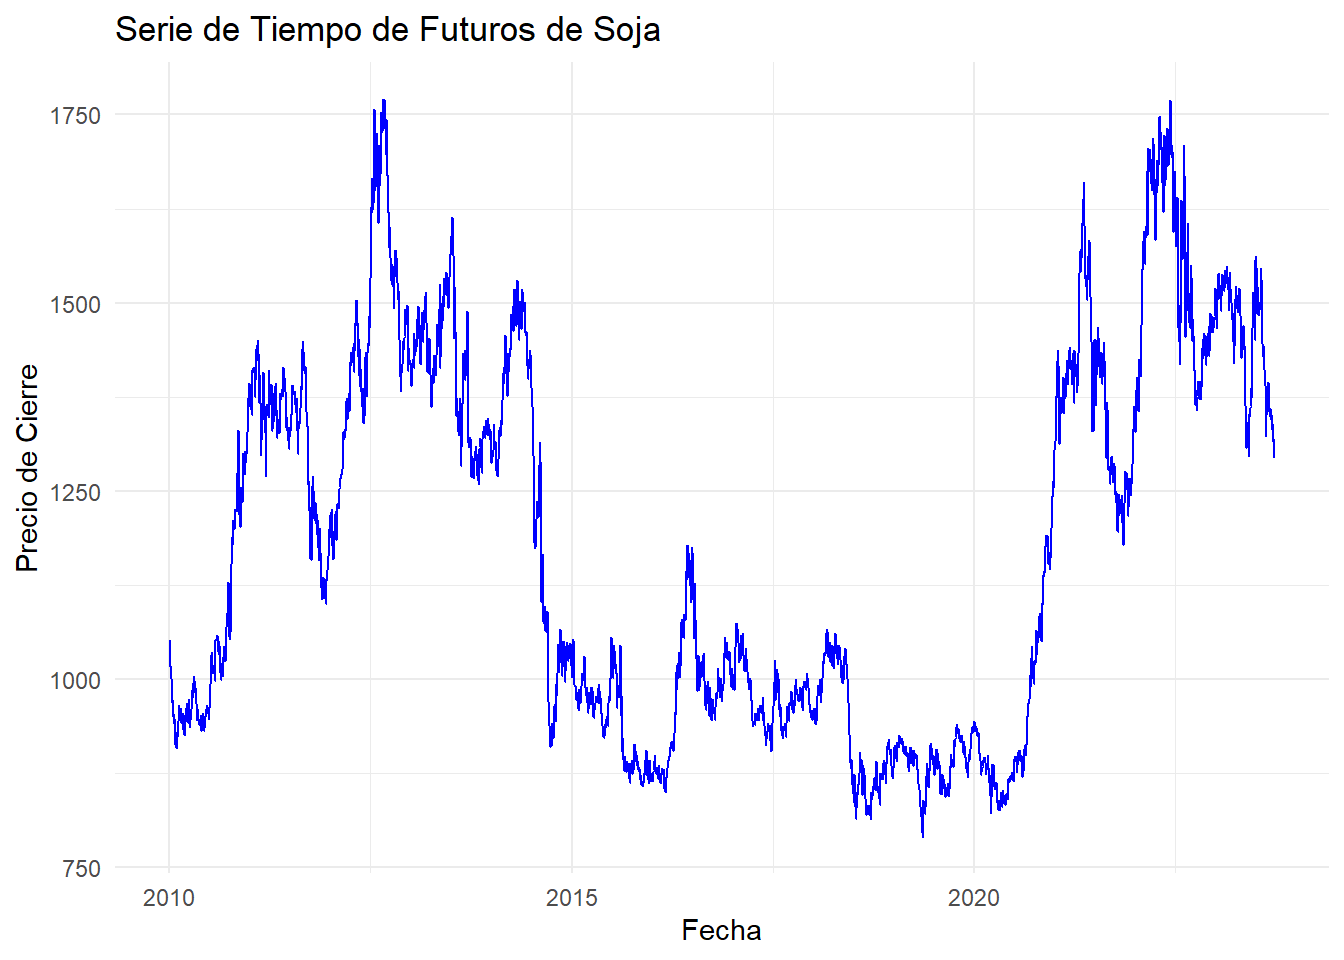
\includegraphics{bookdown-demo_files/figure-latex/unnamed-chunk-9-1.pdf}

\hypertarget{promedio-movil}{%
\chapter{Promedio Movil}\label{promedio-movil}}

Cuando aplicamos un promedio móvil a una serie de tiempo, cada punto de la serie transformada (promediada) es el promedio de un número determinado de puntos anteriores, actuales y futuros de la serie original. Este número de puntos que decides promediar se llama ``ventana'' del promedio móvil.

\begin{Shaded}
\begin{Highlighting}[]
\CommentTok{\# Cargar la biblioteca quantmod}
\FunctionTok{library}\NormalTok{(quantmod)}

\CommentTok{\# Especificar el símbolo para futuros de soja}
\NormalTok{symbol }\OtherTok{\textless{}{-}} \StringTok{"ZS=F"}

\CommentTok{\# Descargar los datos históricos desde el 1 de enero de 2010 hasta hoy}
\FunctionTok{getSymbols}\NormalTok{(symbol, }\AttributeTok{from =} \StringTok{"2010{-}01{-}01"}\NormalTok{, }\AttributeTok{to =} \FunctionTok{Sys.Date}\NormalTok{(), }\AttributeTok{auto.assign =} \ConstantTok{TRUE}\NormalTok{)}
\end{Highlighting}
\end{Shaded}

\begin{verbatim}
## Warning: ZS=F contains missing values. Some functions will not work if objects
## contain missing values in the middle of the series. Consider using na.omit(),
## na.approx(), na.fill(), etc to remove or replace them.
\end{verbatim}

\begin{verbatim}
## [1] "ZS=F"
\end{verbatim}

\begin{Shaded}
\begin{Highlighting}[]
\CommentTok{\# Crear un data frame con la serie de tiempo}
\NormalTok{soybean\_data }\OtherTok{\textless{}{-}} \FunctionTok{data.frame}\NormalTok{(}\AttributeTok{Date =} \FunctionTok{index}\NormalTok{(}\FunctionTok{get}\NormalTok{(symbol)), }
                           \AttributeTok{Open =} \FunctionTok{Op}\NormalTok{(}\FunctionTok{get}\NormalTok{(symbol)),}
                           \AttributeTok{High =} \FunctionTok{Hi}\NormalTok{(}\FunctionTok{get}\NormalTok{(symbol)),}
                           \AttributeTok{Low =} \FunctionTok{Lo}\NormalTok{(}\FunctionTok{get}\NormalTok{(symbol)),}
                           \AttributeTok{Close =} \FunctionTok{Cl}\NormalTok{(}\FunctionTok{get}\NormalTok{(symbol)),}
                           \AttributeTok{Volume =} \FunctionTok{Vo}\NormalTok{(}\FunctionTok{get}\NormalTok{(symbol))}
\NormalTok{                           )}

\CommentTok{\# Eliminar filas con valores NA}
\NormalTok{soybean\_data }\OtherTok{\textless{}{-}} \FunctionTok{na.omit}\NormalTok{(soybean\_data)}

\CommentTok{\# Muestra los primeros registros del data frame}
\CommentTok{\# head(soybean\_data)}
\end{Highlighting}
\end{Shaded}

\begin{Shaded}
\begin{Highlighting}[]
\CommentTok{\# Cargar la biblioteca xts}
\FunctionTok{library}\NormalTok{(xts)}

\CommentTok{\# Crear una serie de tiempo xts a partir del data frame soybean\_data}
\NormalTok{soybean\_xts }\OtherTok{\textless{}{-}} \FunctionTok{xts}\NormalTok{(soybean\_data[, }\SpecialCharTok{{-}}\DecValTok{1}\NormalTok{], }\AttributeTok{order.by =}\NormalTok{ soybean\_data}\SpecialCharTok{$}\NormalTok{Date)}

\CommentTok{\# Verificar la serie de tiempo}
\CommentTok{\# head(soybean\_xts)}
\end{Highlighting}
\end{Shaded}

\begin{Shaded}
\begin{Highlighting}[]
\FunctionTok{library}\NormalTok{(ggplot2)}
\FunctionTok{library}\NormalTok{(TTR)}
\FunctionTok{library}\NormalTok{(scales)}
\end{Highlighting}
\end{Shaded}

\begin{verbatim}
## Warning: package 'scales' was built under R version 4.2.3
\end{verbatim}

\begin{Shaded}
\begin{Highlighting}[]
\CommentTok{\# Convertir el objeto xts a data.frame}
\NormalTok{soybean\_df }\OtherTok{\textless{}{-}} \FunctionTok{as.data.frame}\NormalTok{(soybean\_xts)}
\NormalTok{soybean\_df}\SpecialCharTok{$}\NormalTok{Date }\OtherTok{\textless{}{-}} \FunctionTok{index}\NormalTok{(soybean\_xts)}

\CommentTok{\# Calcular SMA\_200 y SMA\_500}
\NormalTok{soybean\_df}\SpecialCharTok{$}\NormalTok{SMA\_200 }\OtherTok{\textless{}{-}} \FunctionTok{SMA}\NormalTok{(soybean\_df}\SpecialCharTok{$}\NormalTok{ZS.F.Close, }\AttributeTok{n =} \DecValTok{200}\NormalTok{)}
\NormalTok{soybean\_df}\SpecialCharTok{$}\NormalTok{SMA\_500 }\OtherTok{\textless{}{-}} \FunctionTok{SMA}\NormalTok{(soybean\_df}\SpecialCharTok{$}\NormalTok{ZS.F.Close, }\AttributeTok{n =} \DecValTok{500}\NormalTok{)}

\CommentTok{\# Usar ggplot2 para visualizar los datos}
\FunctionTok{ggplot}\NormalTok{(soybean\_df, }\FunctionTok{aes}\NormalTok{(}\AttributeTok{x =}\NormalTok{ Date)) }\SpecialCharTok{+}
  \FunctionTok{geom\_line}\NormalTok{(}\FunctionTok{aes}\NormalTok{(}\AttributeTok{y =}\NormalTok{ ZS.F.Close, }\AttributeTok{color =} \StringTok{\textquotesingle{}Precio de Cierre\textquotesingle{}}\NormalTok{), }\AttributeTok{alpha =} \FloatTok{0.75}\NormalTok{) }\SpecialCharTok{+}
  \FunctionTok{geom\_line}\NormalTok{(}\FunctionTok{aes}\NormalTok{(}\AttributeTok{y =}\NormalTok{ SMA\_200, }\AttributeTok{color =} \StringTok{\textquotesingle{}Promedio Móvil 200\textquotesingle{}}\NormalTok{), }\AttributeTok{size =} \DecValTok{1}\NormalTok{, }\AttributeTok{na.rm =} \ConstantTok{TRUE}\NormalTok{) }\SpecialCharTok{+}
  \FunctionTok{geom\_line}\NormalTok{(}\FunctionTok{aes}\NormalTok{(}\AttributeTok{y =}\NormalTok{ SMA\_500, }\AttributeTok{color =} \StringTok{\textquotesingle{}Promedio Móvil 500\textquotesingle{}}\NormalTok{), }\AttributeTok{size =} \DecValTok{1}\NormalTok{, }\AttributeTok{na.rm =} \ConstantTok{TRUE}\NormalTok{) }\SpecialCharTok{+}
  \FunctionTok{theme\_minimal}\NormalTok{(}\AttributeTok{base\_size =} \DecValTok{15}\NormalTok{) }\SpecialCharTok{+}
  \FunctionTok{labs}\NormalTok{(}\AttributeTok{title =} \StringTok{\textquotesingle{}Serie de Tiempo de Futuros de Soja\textquotesingle{}}\NormalTok{,}
       \AttributeTok{subtitle =} \StringTok{\textquotesingle{}Con Promedios Móviles de 200 y 500 Días\textquotesingle{}}\NormalTok{,}
       \AttributeTok{y =} \StringTok{\textquotesingle{}Precio de Cierre\textquotesingle{}}\NormalTok{) }\SpecialCharTok{+}
  \FunctionTok{theme}\NormalTok{(}\AttributeTok{axis.title.x =} \FunctionTok{element\_blank}\NormalTok{(),}
        \AttributeTok{axis.text.x =} \FunctionTok{element\_text}\NormalTok{(}\AttributeTok{size =} \DecValTok{10}\NormalTok{, }\AttributeTok{angle =} \DecValTok{90}\NormalTok{, }\AttributeTok{vjust =} \FloatTok{0.5}\NormalTok{),}
        \AttributeTok{plot.title =} \FunctionTok{element\_text}\NormalTok{(}\AttributeTok{hjust =} \FloatTok{0.5}\NormalTok{),}
        \AttributeTok{plot.subtitle =} \FunctionTok{element\_text}\NormalTok{(}\AttributeTok{hjust =} \FloatTok{0.5}\NormalTok{),}
        \AttributeTok{legend.position =} \StringTok{"bottom"}\NormalTok{) }\SpecialCharTok{+}
  \FunctionTok{scale\_x\_date}\NormalTok{(}\AttributeTok{date\_breaks =} \StringTok{"1 year"}\NormalTok{, }\AttributeTok{date\_labels =} \StringTok{"\%Y"}\NormalTok{) }\SpecialCharTok{+}
  \FunctionTok{scale\_y\_continuous}\NormalTok{(}\AttributeTok{labels =} \FunctionTok{dollar\_format}\NormalTok{()) }\SpecialCharTok{+}
  \FunctionTok{scale\_color\_manual}\NormalTok{(}\AttributeTok{values =} \FunctionTok{c}\NormalTok{(}\StringTok{\textquotesingle{}Precio de Cierre\textquotesingle{}} \OtherTok{=} \StringTok{\textquotesingle{}blue\textquotesingle{}}\NormalTok{, }\StringTok{\textquotesingle{}Promedio Móvil 200\textquotesingle{}} \OtherTok{=} \StringTok{\textquotesingle{}red\textquotesingle{}}\NormalTok{, }\StringTok{\textquotesingle{}Promedio Móvil 500\textquotesingle{}} \OtherTok{=} \StringTok{\textquotesingle{}green\textquotesingle{}}\NormalTok{),}
                     \AttributeTok{name =} \StringTok{""}\NormalTok{)}
\end{Highlighting}
\end{Shaded}

\begin{verbatim}
## Warning: Using `size` aesthetic for lines was deprecated in ggplot2 3.4.0.
## i Please use `linewidth` instead.
## This warning is displayed once every 8 hours.
## Call `lifecycle::last_lifecycle_warnings()` to see where this warning was
## generated.
\end{verbatim}

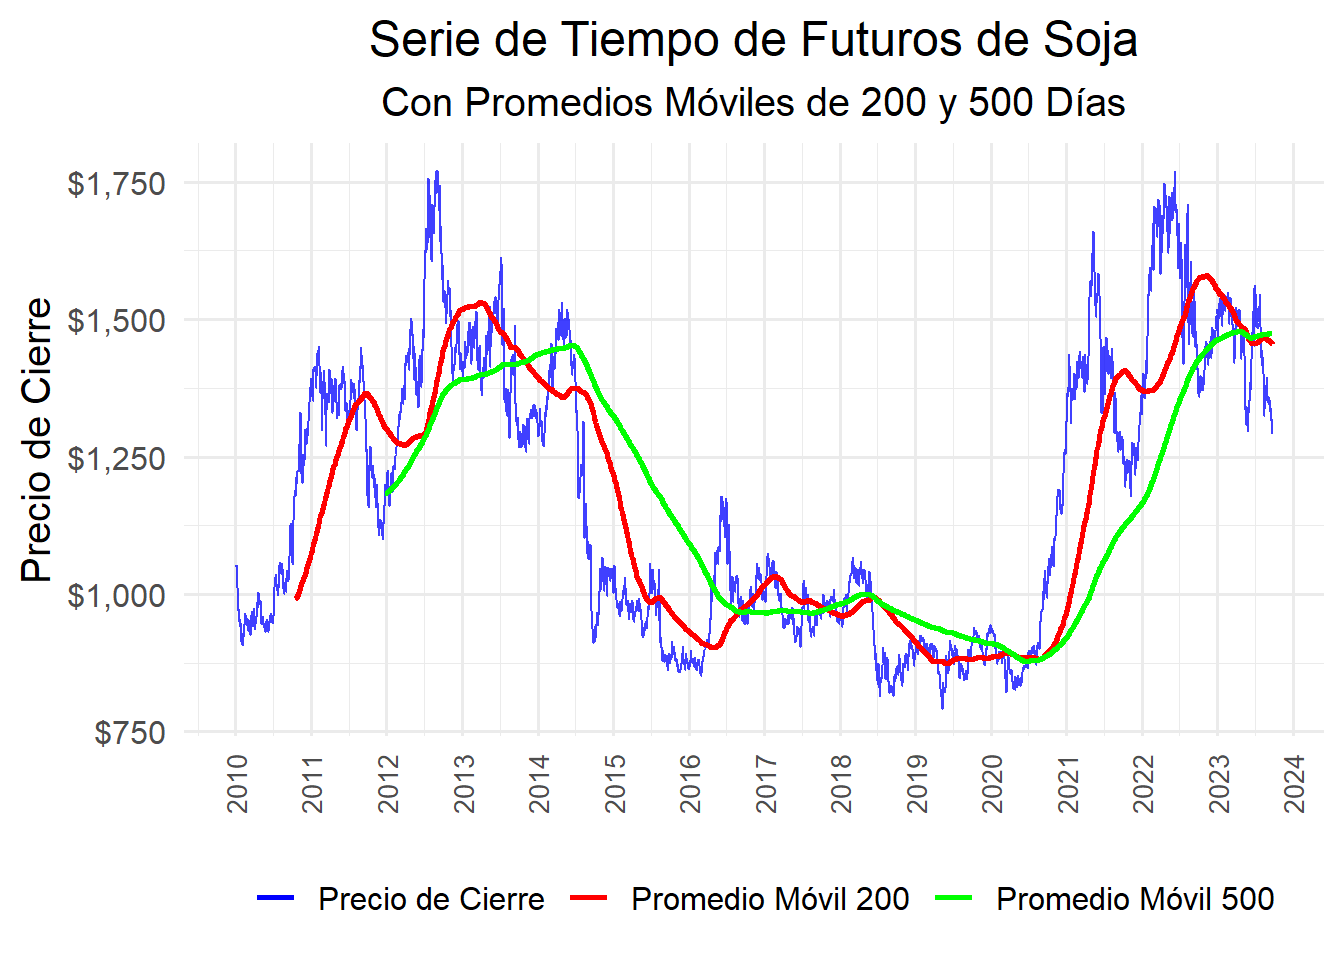
\includegraphics{bookdown-demo_files/figure-latex/unnamed-chunk-12-1.pdf}

Observaciones:

Entre los años 2013 y mediados del 2014 se puede ver cambios en la tendencia de la serie de tiempo de futuros de la soya, tamto para el promedio movil de 200 días, como para el de 500 días el cual es mas marcado.

Entre los años 2021 y mediados del 2023 se puede ver cambios en la tendencia de la serie de tiempo de futuros de la soya, tamto para el promedio movil de 200 días, como para el de 500 días el cual es mas marcado.Se podria llegar a validar por medio de un mayor estudio de este tiempo si la afectación fue causada por el desarrollo de la pandemia del covid-19 la cul inicio en marzo de 2020 e inicio a retrocer en Agosto de 2021 cuando se inicio el uso de las vacunas.

Al suavizar las fluctuaciones menores, a traves de los promedios móviles se logro resaltar las tendencias subyacentes en los datos.

\hypertarget{rezago}{%
\chapter{Rezago}\label{rezago}}

El concepto de rezago es fundamental para analizar y modelar series de tiempo porque permite entender cómo los valores pasados pueden influir en los valores presentes o futuros de la serie. Al analizar los rezagos, podemos identificar patrones, hacer predicciones más precisas y entender mejor la dinámica subyacente de los datos.

\begin{Shaded}
\begin{Highlighting}[]
\CommentTok{\# Sin cargar la librería dplyr para evitar conflictos}
\NormalTok{datos\_lag }\OtherTok{\textless{}{-}} \FunctionTok{data.frame}\NormalTok{(}
  \AttributeTok{Close =} \FunctionTok{as.numeric}\NormalTok{(}\FunctionTok{coredata}\NormalTok{(soybean\_xts)),}
  \AttributeTok{Lag =} \FunctionTok{as.numeric}\NormalTok{(}\FunctionTok{coredata}\NormalTok{(stats}\SpecialCharTok{::}\FunctionTok{lag}\NormalTok{(soybean\_xts))) }\CommentTok{\# Usar stats::lag para evitar conflictos}
\NormalTok{)}

\CommentTok{\# Comprobando que ambos vectores tengan la misma longitud}
\FunctionTok{stopifnot}\NormalTok{(}\FunctionTok{length}\NormalTok{(datos\_lag}\SpecialCharTok{$}\NormalTok{Close) }\SpecialCharTok{==} \FunctionTok{length}\NormalTok{(datos\_lag}\SpecialCharTok{$}\NormalTok{Lag))  }\CommentTok{\# Detiene la ejecución si no son TRUE}

\CommentTok{\# Crear el gráfico de rezago con ggplot2}
\FunctionTok{library}\NormalTok{(ggplot2)}
\FunctionTok{ggplot}\NormalTok{(datos\_lag, }\FunctionTok{aes}\NormalTok{(}\AttributeTok{x=}\NormalTok{Lag, }\AttributeTok{y=}\NormalTok{Close)) }\SpecialCharTok{+}
  \FunctionTok{geom\_point}\NormalTok{(}\FunctionTok{aes}\NormalTok{(}\AttributeTok{color =}\NormalTok{ Close), }\AttributeTok{alpha=}\FloatTok{0.6}\NormalTok{) }\SpecialCharTok{+}
  \FunctionTok{geom\_smooth}\NormalTok{(}\AttributeTok{method =} \StringTok{\textquotesingle{}lm\textquotesingle{}}\NormalTok{, }\AttributeTok{se =} \ConstantTok{FALSE}\NormalTok{, }\AttributeTok{color=}\StringTok{"blue"}\NormalTok{, }\AttributeTok{linetype=}\StringTok{"dashed"}\NormalTok{) }\SpecialCharTok{+}
  \FunctionTok{scale\_color\_gradient}\NormalTok{(}\AttributeTok{low=}\StringTok{"red"}\NormalTok{, }\AttributeTok{high=}\StringTok{"green"}\NormalTok{) }\SpecialCharTok{+}
  \FunctionTok{theme\_minimal}\NormalTok{() }\SpecialCharTok{+}
  \FunctionTok{labs}\NormalTok{(}\AttributeTok{title=}\StringTok{"Gráfico de Rezago para Precio de Cierre"}\NormalTok{, }\AttributeTok{x=}\StringTok{"Rezago 1"}\NormalTok{, }\AttributeTok{y=}\StringTok{"Precio de Cierre"}\NormalTok{) }\SpecialCharTok{+}
  \FunctionTok{theme}\NormalTok{(}\AttributeTok{legend.position=}\StringTok{"none"}\NormalTok{)}
\end{Highlighting}
\end{Shaded}

\begin{verbatim}
## `geom_smooth()` using formula = 'y ~ x'
\end{verbatim}

\begin{verbatim}
## Warning: Removed 5 rows containing non-finite values (`stat_smooth()`).
\end{verbatim}

\begin{verbatim}
## Warning: Removed 5 rows containing missing values (`geom_point()`).
\end{verbatim}

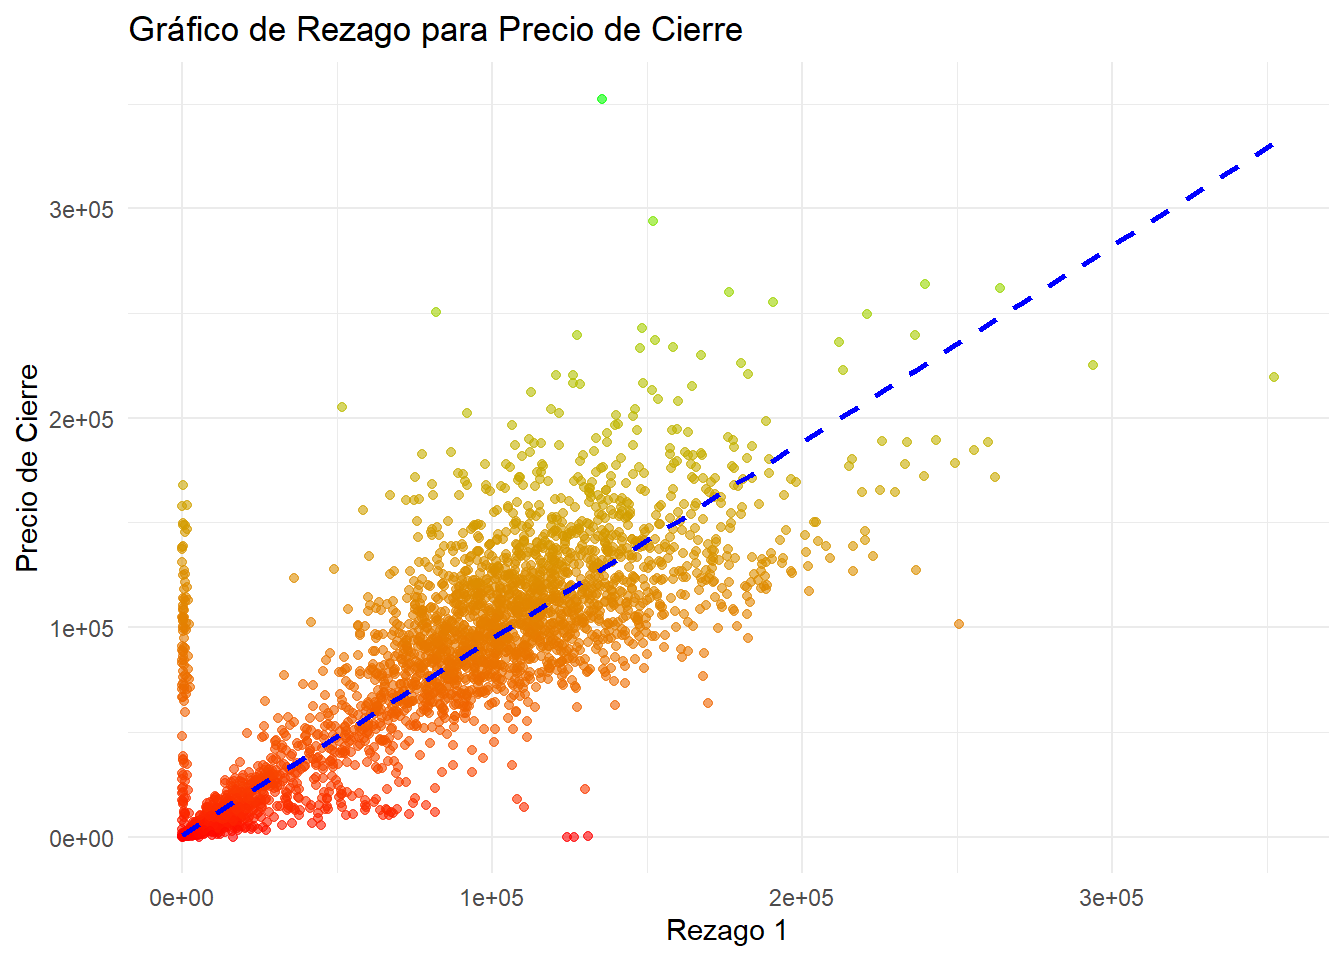
\includegraphics{bookdown-demo_files/figure-latex/unnamed-chunk-13-1.pdf}

Se ve un patrón claro o una agrupación de puntos en el gráfico de rezago 1, por lo tanto es probable que exista una autocorrelación significativa. Se puede considerar modelos de series de tiempo como ARIMA que toman en cuenta la autocorrelación para hacer predicciones más precisas de ser necesario.

\hypertarget{descomposicion}{%
\chapter{Descomposicion}\label{descomposicion}}

Se refiere a los patrones o tendencias que se repiten a intervalos regulares, como cada día, mes, trimestre o año, dependiendo de la frecuencia de los datos. En otras palabras, es como un ciclo que se repite en el tiempo.

DESCOMPOSICION

Con la funcion decompose podemos hallar la:

Observed: Serie de tiempo original.

Tendencia (trend): Muestra la dirección general en la que se mueven los datos a largo plazo, sin tener en cuenta las fluctuaciones estacionales o irregulares.

Estacionalidad (seasonal): Representa las fluctuaciones que ocurren en intervalos regulares, como los cambios diarios, mensuales o anuales, debido a la estacionalidad.

Error o Residuo (random): Es la parte de la serie de tiempo que no se puede atribuir ni a la tendencia ni a la estacionalidad. Captura la variabilidad en los datos que no se puede explicar por los otros dos componentes.

\begin{Shaded}
\begin{Highlighting}[]
\CommentTok{\# Convertir a objeto ts, aquí supondré que tienes datos diarios.}
\NormalTok{frecuencia }\OtherTok{\textless{}{-}} \DecValTok{365}  \CommentTok{\# (12 para mensual, 4 para trimestral, etc.)}
\NormalTok{soybean\_ts }\OtherTok{\textless{}{-}} \FunctionTok{ts}\NormalTok{(soybean\_xts[, }\StringTok{"ZS.F.Close"}\NormalTok{], }\AttributeTok{frequency =}\NormalTok{ frecuencia)}

\CommentTok{\# Utilizar decompose}
\NormalTok{soybean\_decomposed }\OtherTok{\textless{}{-}} \FunctionTok{decompose}\NormalTok{(soybean\_ts)}
\FunctionTok{plot}\NormalTok{(soybean\_decomposed)}
\end{Highlighting}
\end{Shaded}

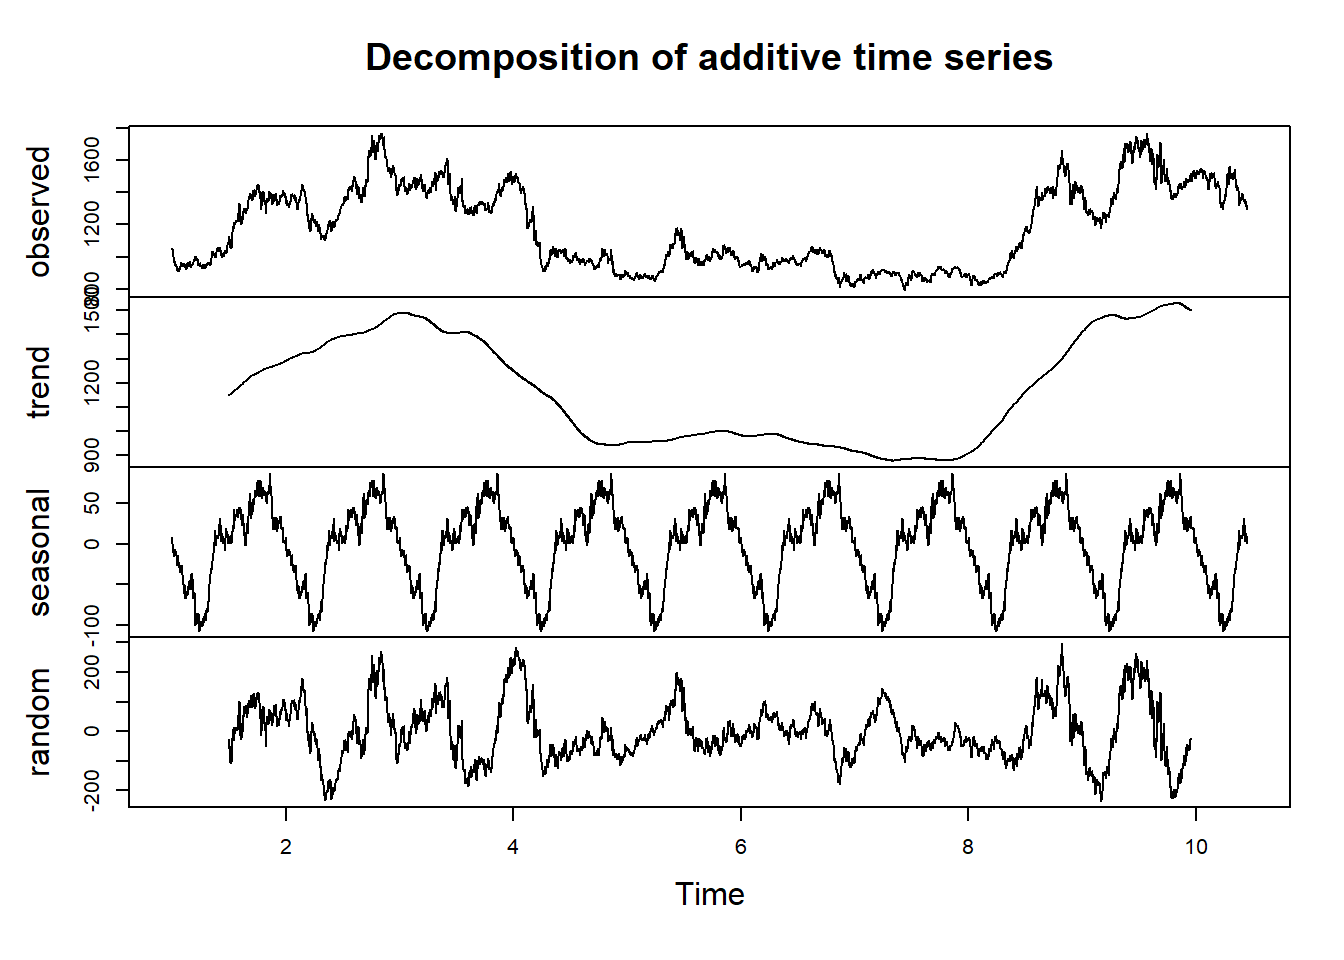
\includegraphics{bookdown-demo_files/figure-latex/unnamed-chunk-14-1.pdf}
Al validar el componenete estacional de la serie por separado, como se ve en la siguiente imagen:

\begin{Shaded}
\begin{Highlighting}[]
\CommentTok{\# Extraer el componente estacional y convertir el tiempo en fecha}
\NormalTok{seasonal\_df }\OtherTok{\textless{}{-}} \FunctionTok{data.frame}\NormalTok{(}
  \AttributeTok{Date =} \FunctionTok{as.Date}\NormalTok{(}\FunctionTok{index}\NormalTok{(soybean\_xts)),}
  \AttributeTok{Seasonal =} \FunctionTok{as.numeric}\NormalTok{(soybean\_decomposed}\SpecialCharTok{$}\NormalTok{seasonal)}
\NormalTok{)}

\CommentTok{\# Eliminar las filas con NA en el componente estacional (pueden aparecer dependiendo del método de descomposición)}
\NormalTok{seasonal\_df }\OtherTok{\textless{}{-}}\NormalTok{ seasonal\_df[}\SpecialCharTok{!}\FunctionTok{is.na}\NormalTok{(seasonal\_df}\SpecialCharTok{$}\NormalTok{Seasonal), ]}
\end{Highlighting}
\end{Shaded}

\begin{Shaded}
\begin{Highlighting}[]
\FunctionTok{library}\NormalTok{(ggplot2)}

\FunctionTok{ggplot}\NormalTok{(seasonal\_df, }\FunctionTok{aes}\NormalTok{(}\AttributeTok{x=}\NormalTok{Date, }\AttributeTok{y=}\NormalTok{Seasonal)) }\SpecialCharTok{+}
  \FunctionTok{geom\_line}\NormalTok{(}\AttributeTok{color=}\StringTok{"blue"}\NormalTok{) }\SpecialCharTok{+}
  \FunctionTok{theme\_minimal}\NormalTok{() }\SpecialCharTok{+}
  \FunctionTok{labs}\NormalTok{(}\AttributeTok{title=}\StringTok{"Componente Estacional de la Serie Temporal"}\NormalTok{, }\AttributeTok{x=}\StringTok{"Fecha"}\NormalTok{, }\AttributeTok{y=}\StringTok{"Estacionalidad"}\NormalTok{) }\SpecialCharTok{+}
  \FunctionTok{theme}\NormalTok{(}\AttributeTok{legend.position=}\StringTok{"none"}\NormalTok{)}
\end{Highlighting}
\end{Shaded}

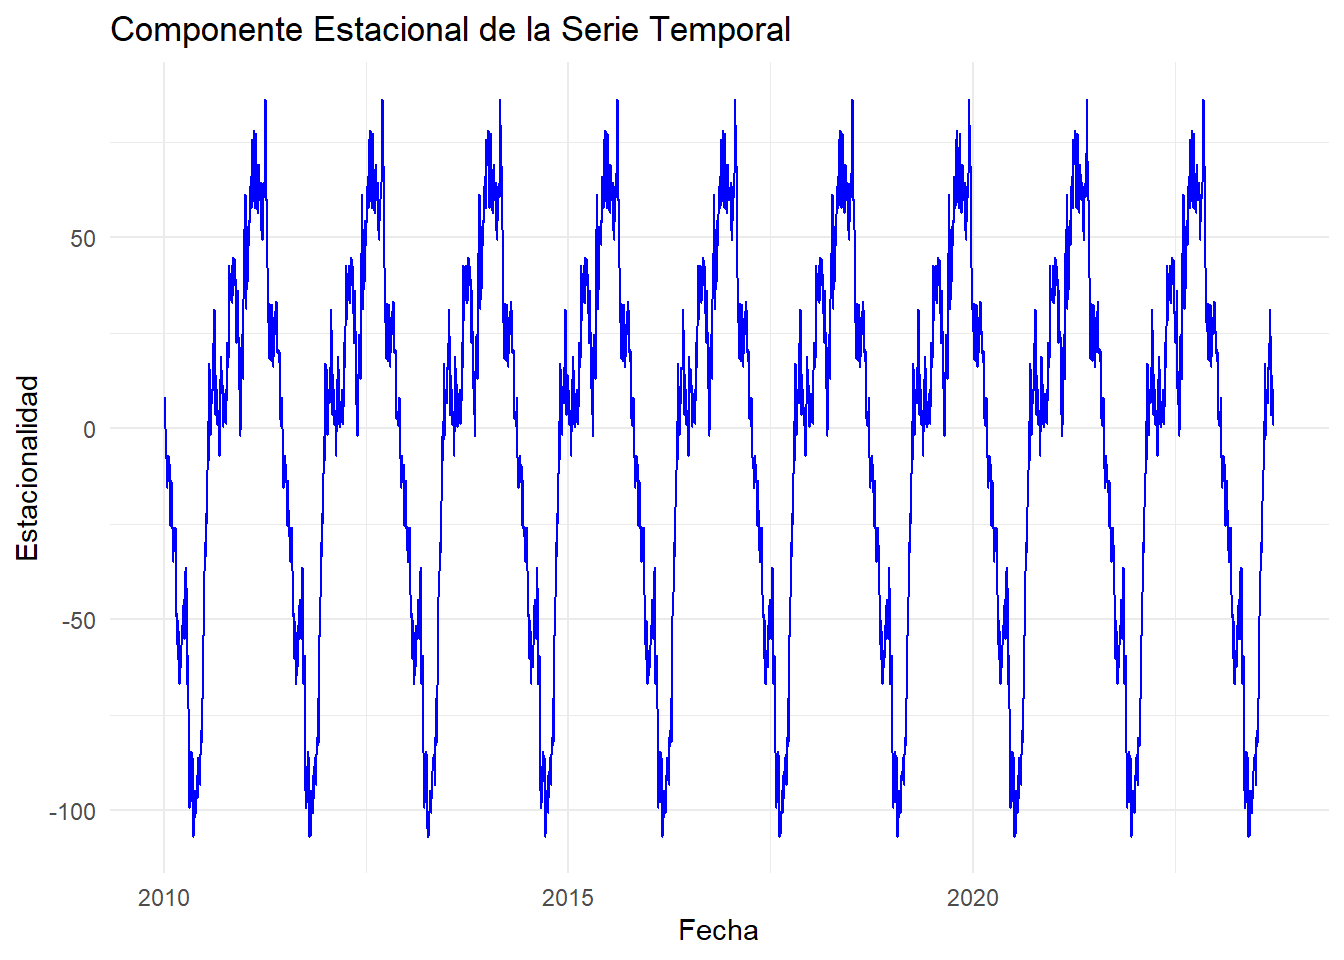
\includegraphics{bookdown-demo_files/figure-latex/unnamed-chunk-16-1.pdf}
Podemos deducir que la serie de tiempo de los precios del aceite de soya:

\begin{enumerate}
\def\labelenumi{\arabic{enumi}.}
\item
  Muestra patrones claros y consistentes, esto sugiere que la serie temporal tiene ciclos regulares que se repiten a intervalos fijos.
\item
  Se pueden identificar en qué momentos del ciclo tienden a ocurrir los valores altos y bajos de la serie.
\end{enumerate}

\hypertarget{estacionariedad}{%
\chapter{Estacionariedad}\label{estacionariedad}}

La prueba de Dickey-Fuller, específicamente el test ADF (Augmented Dickey-Fuller), es una prueba estadística utilizada para determinar si una serie temporal tiene una raíz unitaria, es decir, si es no estacionaria y presenta alguna forma de estructura temporal como una tendencia o una estacionalidad.

Vamos a comprobar mediante esta prueba si es o no estacionaria la serie de tiempo del precio del aceite de soya.

\begin{Shaded}
\begin{Highlighting}[]
\CommentTok{\# Cargar el paquete necesario}
\FunctionTok{library}\NormalTok{(tseries)}
\end{Highlighting}
\end{Shaded}

\begin{verbatim}
## Warning: package 'tseries' was built under R version 4.2.3
\end{verbatim}

\begin{Shaded}
\begin{Highlighting}[]
\CommentTok{\# Supón que tienes una serie temporal llamada \textquotesingle{}mi\_serie\textquotesingle{}}
\CommentTok{\# Realizar la prueba de Dickey{-}Fuller Aumentada}
\NormalTok{resultado\_adf }\OtherTok{\textless{}{-}} \FunctionTok{adf.test}\NormalTok{(soybean\_ts)}

\CommentTok{\# Imprimir el resultado}
\FunctionTok{print}\NormalTok{(resultado\_adf)}
\end{Highlighting}
\end{Shaded}

\begin{verbatim}
## 
##  Augmented Dickey-Fuller Test
## 
## data:  soybean_ts
## Dickey-Fuller = -2.0292, Lag order = 15, p-value = 0.566
## alternative hypothesis: stationary
\end{verbatim}

Cuando hacemos una prueba como esta, estamos tratando de averiguar si la serie de tiempo es ``estacionaria'' o no. Una serie estacionaria es aquella cuyas propiedades, como la media y la varianza, no cambian con el tiempo.

En esta prueba, tenemos algo llamado valor p, que es como un termómetro que nos dice qué tan seguros estamos de si la serie de tiempo es estacionaria o no. Un valor p pequeño (menor que 0.05) nos dice: ``La serie es estacionaria''. Un valor p grande (mayor que 0.05) nos dice: ``La serie no es estacionaria''.

En este caso, el valor p es 0.5657, que es bastante grande, así que, la serie de tiempo no es estacionaria.

\hypertarget{diferenciacion}{%
\chapter{Diferenciacion}\label{diferenciacion}}

Diferenciar una serie temporal es un proceso utilizado para hacer que una serie no estacionaria se vuelva estacionaria. La idea es transformar la serie de datos para estabilizar la media de la serie temporal, eliminando tendencias y efectos estacionales. En otras palabras, se busca que las propiedades de la serie (como la media y la varianza) no cambien con el tiempo.

\begin{Shaded}
\begin{Highlighting}[]
\CommentTok{\# Inicializa un contador para las diferenciaciones}
\NormalTok{diferencias }\OtherTok{\textless{}{-}} \DecValTok{0}

\CommentTok{\# Realiza el test ADF y verifica la estacionariedad}
\ControlFlowTok{while}\NormalTok{(}\ConstantTok{TRUE}\NormalTok{) \{}
\NormalTok{  p\_value }\OtherTok{\textless{}{-}} \FunctionTok{adf.test}\NormalTok{(soybean\_ts)}\SpecialCharTok{$}\NormalTok{p.value}
  \FunctionTok{cat}\NormalTok{(}\StringTok{"Número de diferencias:"}\NormalTok{, diferencias, }\StringTok{"{-} Valor p:"}\NormalTok{, p\_value, }\StringTok{"}\SpecialCharTok{\textbackslash{}n}\StringTok{"}\NormalTok{)}
  
  \CommentTok{\# Si el valor p es menor que 0.05, la serie es estacionaria, y puedes salir del bucle.}
  \ControlFlowTok{if}\NormalTok{(p\_value }\SpecialCharTok{\textless{}} \FloatTok{0.05}\NormalTok{) \{}
    \FunctionTok{cat}\NormalTok{(}\StringTok{"La serie se volvió estacionaria después de"}\NormalTok{, diferencias, }\StringTok{"diferenciaciones.}\SpecialCharTok{\textbackslash{}n}\StringTok{"}\NormalTok{)}
    \ControlFlowTok{break}
\NormalTok{  \}}
  
  \CommentTok{\# Si has llegado al final de la serie, sal del bucle}
  \ControlFlowTok{if}\NormalTok{(}\FunctionTok{length}\NormalTok{(soybean\_ts) }\SpecialCharTok{\textless{}=} \DecValTok{1}\NormalTok{) \{}
    \FunctionTok{cat}\NormalTok{(}\StringTok{"La serie no se volvió estacionaria después de diferenciar.}\SpecialCharTok{\textbackslash{}n}\StringTok{"}\NormalTok{)}
    \ControlFlowTok{break}
\NormalTok{  \}}
  
  \CommentTok{\# Si no es estacionaria, diferenciar la serie una vez más y continuar el bucle.}
\NormalTok{  soybean\_ts }\OtherTok{\textless{}{-}} \FunctionTok{diff}\NormalTok{(soybean\_ts)}
\NormalTok{  diferencias }\OtherTok{\textless{}{-}}\NormalTok{ diferencias }\SpecialCharTok{+} \DecValTok{1}
\NormalTok{\}}
\end{Highlighting}
\end{Shaded}

\begin{verbatim}
## Número de diferencias: 0 - Valor p: 0.5659563
\end{verbatim}

\begin{verbatim}
## Warning in adf.test(soybean_ts): p-value smaller than printed p-value
\end{verbatim}

\begin{verbatim}
## Número de diferencias: 1 - Valor p: 0.01 
## La serie se volvió estacionaria después de 1 diferenciaciones.
\end{verbatim}

Conclusión:

Antes de realizar cualquier diferenciación (d = 0), el valor p de la prueba de Dickey-Fuller Aumentada es 0.5657422, lo que es mayor que 0.05. Por lo tanto, no puedes rechazar la hipótesis nula de que existe una raíz unitaria, y se concluye que la serie original no es estacionaria.

Después de diferenciar la serie una vez (d = 1), el valor p de la prueba de Dickey-Fuller Aumentada es 0.01, lo cual es menor que 0.05.

La serie de tiempo original no es estacionaria, pero después de realizar una diferenciación, la serie resultante sí es estacionaria.

Fue necesario transformarla o diferenciarla para eliminar la tendencia y estabilizar la varianza, antes de aplicar modelos de series temporales como ARIMA.

\hypertarget{holter-winter}{%
\chapter{Holter-Winter}\label{holter-winter}}

La metodología Holt-Winters, también conocida como triple suavizado exponencial, es útil para series de tiempo con componentes de tendencia y estacionalidad.

\begin{Shaded}
\begin{Highlighting}[]
\FunctionTok{library}\NormalTok{(forecast)  }\CommentTok{\# Necesario para pronosticar con el modelo Holt{-}Winters}
\end{Highlighting}
\end{Shaded}

\begin{verbatim}
## Warning: package 'forecast' was built under R version 4.2.3
\end{verbatim}

\begin{Shaded}
\begin{Highlighting}[]
\CommentTok{\# Ajustar el modelo Holt{-}Winters}
\NormalTok{hw\_model }\OtherTok{\textless{}{-}} \FunctionTok{HoltWinters}\NormalTok{(soybean\_ts)}
\CommentTok{\# Visualizar componentes del modelo}
\FunctionTok{plot}\NormalTok{(hw\_model)}
\end{Highlighting}
\end{Shaded}

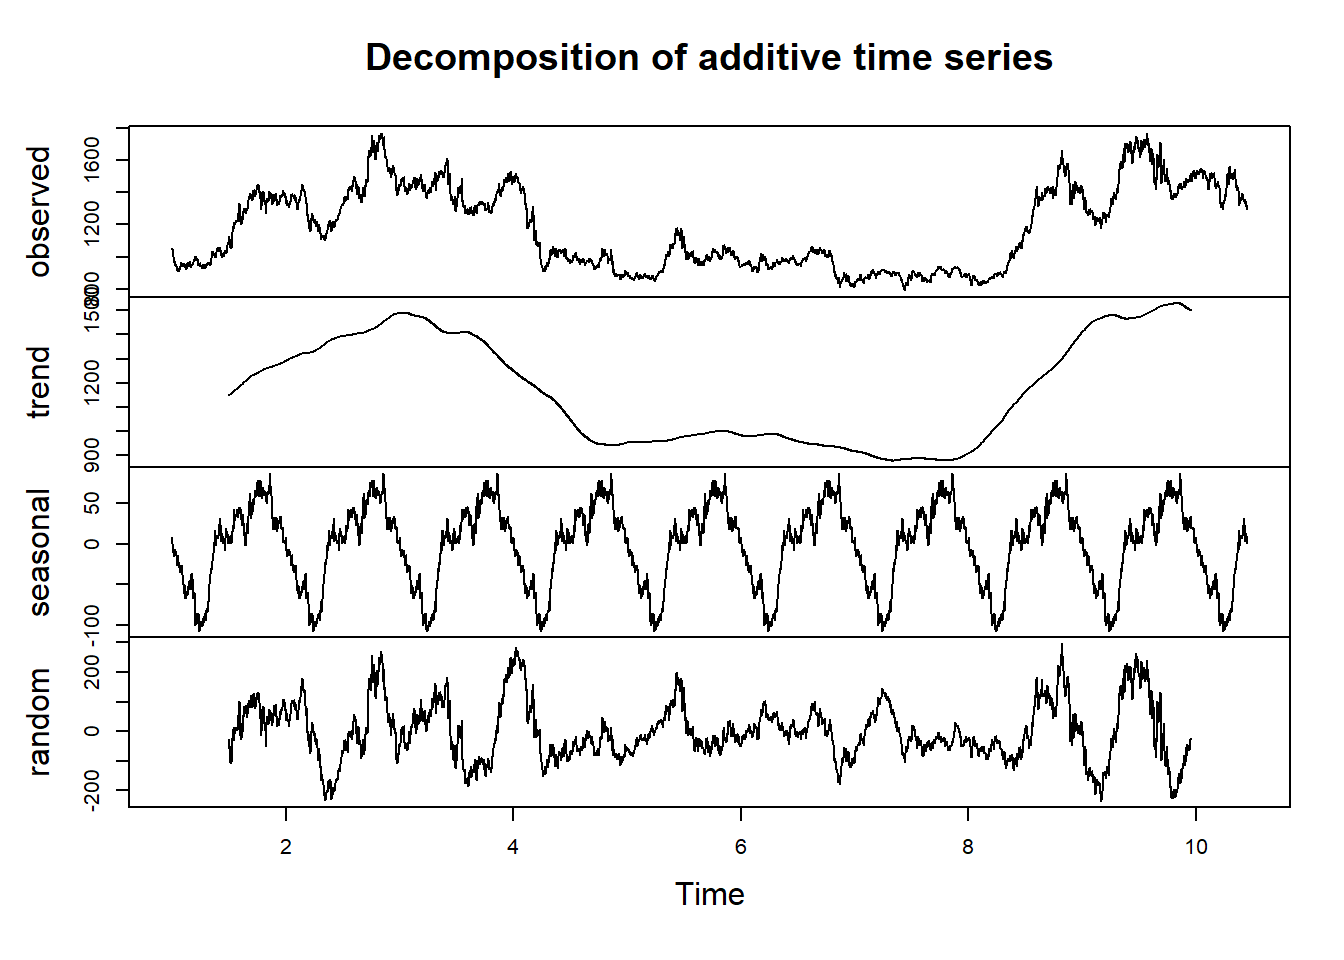
\includegraphics{bookdown-demo_files/figure-latex/unnamed-chunk-19-1.pdf}

\begin{Shaded}
\begin{Highlighting}[]
\CommentTok{\# Pronosticar los siguientes 30 días (o la cantidad que desees)}
\FunctionTok{library}\NormalTok{(forecast)}
\NormalTok{hw\_forecast }\OtherTok{\textless{}{-}} \FunctionTok{forecast}\NormalTok{(hw\_model, }\AttributeTok{h =} \DecValTok{30}\NormalTok{)  }\CommentTok{\# Cambia 30 por el número de periodos que quieras pronosticar}
\FunctionTok{plot}\NormalTok{(hw\_forecast)}
\end{Highlighting}
\end{Shaded}

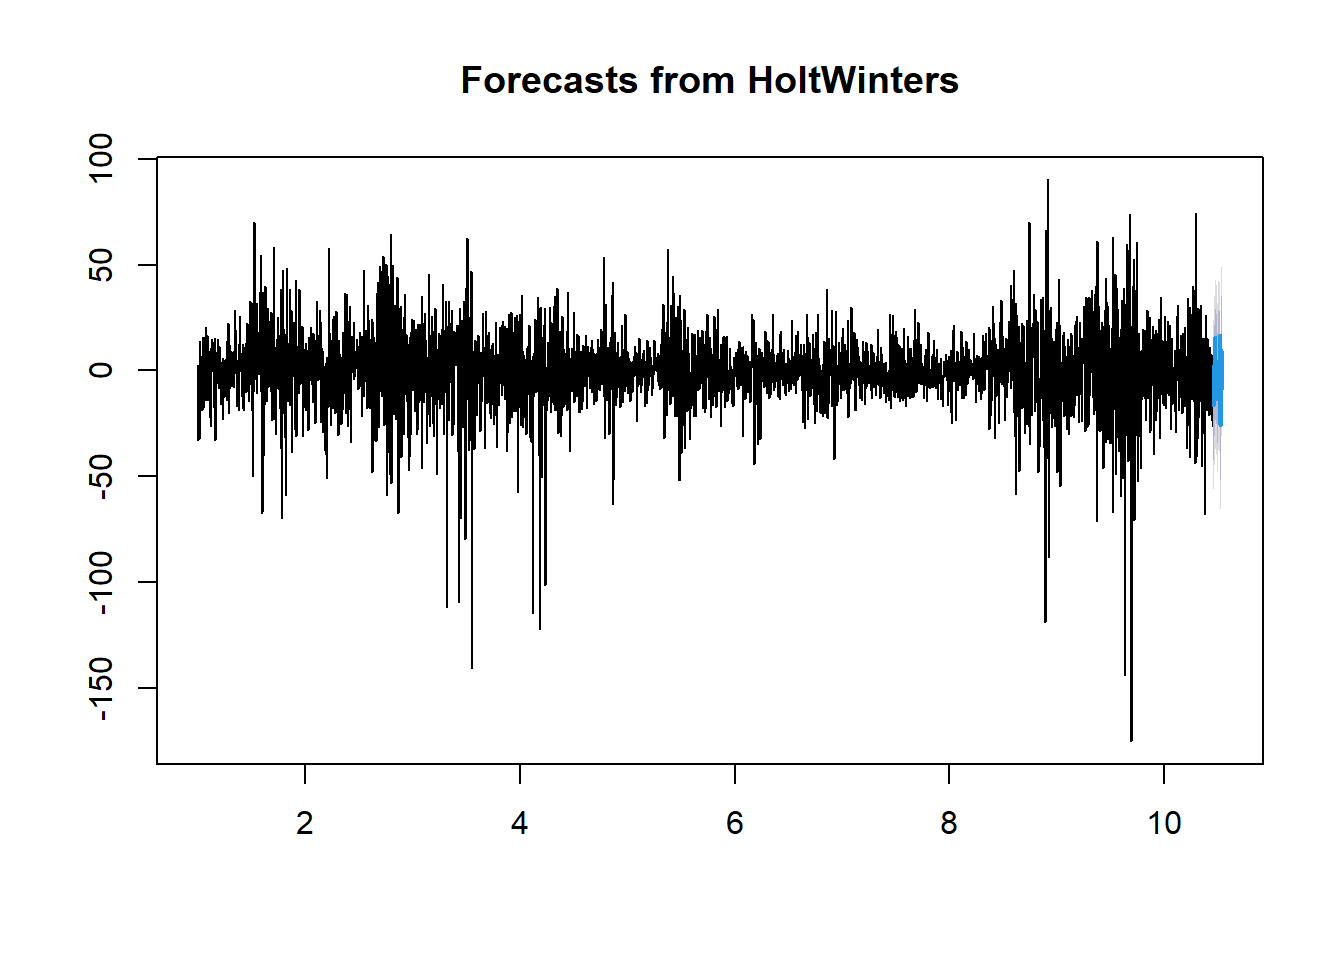
\includegraphics{bookdown-demo_files/figure-latex/unnamed-chunk-20-1.pdf}

\begin{Shaded}
\begin{Highlighting}[]
\CommentTok{\# Revisar detalles del modelo y del pronóstico}
\FunctionTok{summary}\NormalTok{(hw\_model)}
\end{Highlighting}
\end{Shaded}

\begin{verbatim}
##              Length Class  Mode     
## fitted       12344  mts    numeric  
## x             3451  ts     numeric  
## alpha            1  -none- numeric  
## beta             1  -none- numeric  
## gamma            1  -none- numeric  
## coefficients   367  -none- numeric  
## seasonal         1  -none- character
## SSE              1  -none- numeric  
## call             2  -none- call
\end{verbatim}

\begin{Shaded}
\begin{Highlighting}[]
\FunctionTok{summary}\NormalTok{(hw\_forecast)}
\end{Highlighting}
\end{Shaded}

\begin{verbatim}
## 
## Forecast method: HoltWinters
## 
## Model Information:
## Holt-Winters exponential smoothing with trend and additive seasonal component.
## 
## Call:
## HoltWinters(x = soybean_ts)
## 
## Smoothing parameters:
##  alpha: 0.001514729
##  beta : 0
##  gamma: 0.3525257
## 
## Coefficients:
##               [,1]
## a     -1.956309078
## b     -0.001484417
## s1   -14.281107092
## s2     4.583967378
## s3     2.918793461
## s4    -2.789000303
## s5    16.443962574
## s6    10.324885438
## s7    17.933824650
## s8     5.227538747
## s9   -11.332855543
## s10    0.963450269
## s11    3.006261120
## s12    1.803077568
## s13   -3.372927065
## s14   -0.286317331
## s15   -6.262594113
## s16    0.462270912
## s17    6.239814363
## s18    4.799396311
## s19   -4.146463534
## s20   -9.703369870
## s21    3.719285245
## s22    6.924404043
## s23   -0.322275263
## s24   18.803061258
## s25  -23.827895496
## s26   11.564351838
## s27   -6.134173103
## s28   11.365624802
## s29    6.817464887
## s30   -6.404630586
## s31    1.182661250
## s32    0.668715285
## s33   18.859190485
## s34   10.309870898
## s35  -16.759165840
## s36    7.158833838
## s37   19.005655277
## s38   -4.237196909
## s39    2.587979255
## s40   10.746441111
## s41    5.349276176
## s42    8.702955612
## s43    3.630210455
## s44  -10.924486006
## s45   -1.965773652
## s46    0.945128150
## s47   10.236617208
## s48    4.125157663
## s49   -5.219359050
## s50   -6.619939049
## s51  -21.193379399
## s52   12.984113174
## s53    7.723779327
## s54   16.780446641
## s55   -0.162082988
## s56   -4.704009268
## s57  -18.571373311
## s58  -14.156340320
## s59  -12.703585137
## s60   15.060195235
## s61   17.053278484
## s62    7.283202539
## s63  -20.781088204
## s64    1.985091856
## s65    6.134516491
## s66  -52.342262066
## s67   14.417589393
## s68   -8.419114089
## s69   -9.274947091
## s70   -6.024054427
## s71   11.069394177
## s72    2.827748510
## s73   27.514726331
## s74   18.077345868
## s75   14.726646620
## s76    8.709806740
## s77  -16.219917936
## s78   -8.324257848
## s79   -1.276683386
## s80   30.529461754
## s81   10.201361073
## s82   -0.137173236
## s83   26.177548608
## s84   -1.444200669
## s85   12.811192394
## s86  -13.431936931
## s87  -60.820413303
## s88   -6.669146357
## s89   11.422568416
## s90    7.684110273
## s91  -10.000892420
## s92   14.125307650
## s93   19.214550159
## s94    0.538559388
## s95   -2.874808287
## s96   17.784586776
## s97  -28.230526832
## s98    0.771334656
## s99   -0.498737674
## s100  -5.881432758
## s101  12.774001259
## s102  -5.361351292
## s103 -10.687103592
## s104   0.422286320
## s105   0.428605345
## s106  38.638905544
## s107 -10.554984367
## s108  -7.766191307
## s109 -14.398407981
## s110  -2.773298946
## s111   9.088082546
## s112   2.486688811
## s113 -13.372005559
## s114   1.293653550
## s115  -5.531005265
## s116   0.145331133
## s117   7.021019182
## s118   6.308660885
## s119   4.272316145
## s120 -10.798436363
## s121  13.075192573
## s122   2.340166812
## s123   1.586274216
## s124  -7.783044624
## s125   4.557803654
## s126   0.887639104
## s127  10.302310196
## s128   1.842563088
## s129   3.103742116
## s130  -3.664794016
## s131   5.185257531
## s132  -1.535217711
## s133  -0.959775839
## s134   8.513180682
## s135   6.917627484
## s136 -20.942086358
## s137   1.534178685
## s138  -3.488710973
## s139   2.785545805
## s140  -5.993975793
## s141   8.962741704
## s142  11.072889880
## s143   3.115042078
## s144  -7.254170594
## s145   8.589108499
## s146   5.511724446
## s147   3.791181047
## s148  16.773516706
## s149  -9.351130261
## s150   2.788854437
## s151   3.402704414
## s152  -1.043280871
## s153  -5.583551155
## s154  -6.439560106
## s155  -1.968067528
## s156  -2.509718145
## s157  -9.727873812
## s158   1.844410463
## s159  -3.993091601
## s160 -17.642176946
## s161  18.934914731
## s162   9.982863021
## s163 -17.415211021
## s164   2.594499451
## s165  -1.241668740
## s166  -5.701246552
## s167  14.042612941
## s168   6.085406103
## s169  19.205564134
## s170  -8.556902915
## s171   8.126886625
## s172 -19.076516734
## s173   0.233830853
## s174   3.985080649
## s175  -2.589684926
## s176  13.189264317
## s177   3.124277141
## s178   1.130484976
## s179   0.337039064
## s180   4.944833119
## s181   3.277836557
## s182   3.585703609
## s183   4.034900177
## s184 -16.129832582
## s185  -7.699941984
## s186   0.768739710
## s187  15.056250629
## s188   5.622358119
## s189   3.004545292
## s190  -1.539276651
## s191   6.943821408
## s192  -4.631462369
## s193   2.954004611
## s194  -5.444204562
## s195   1.838126421
## s196  -0.438287461
## s197  -1.747127540
## s198  -6.973611058
## s199   4.701637451
## s200  15.673685991
## s201 -15.214330625
## s202   6.054159010
## s203  -2.668629163
## s204 -11.320034526
## s205  -1.705173481
## s206  -0.139890969
## s207   5.294734477
## s208  -1.728024085
## s209   8.473214930
## s210  -1.797720807
## s211  -0.484639902
## s212   3.589397584
## s213  -2.538577090
## s214  -3.400238313
## s215   1.013407215
## s216  -3.034096139
## s217  11.362873970
## s218  -1.565963913
## s219   2.504461213
## s220  -5.755246471
## s221  -4.765770508
## s222  -5.848807681
## s223   5.890564209
## s224   3.341836926
## s225  -0.123618413
## s226   9.129945747
## s227  -2.768004714
## s228  -1.386249039
## s229  -2.245768072
## s230  -0.738299646
## s231  -3.822233531
## s232   1.577293282
## s233  -9.767695446
## s234  -1.406284490
## s235  -7.984184425
## s236   6.660660256
## s237  -9.008938635
## s238  -5.462878289
## s239  -7.774807820
## s240   4.689961531
## s241   0.316274044
## s242   8.338475159
## s243   3.274439073
## s244   1.541567724
## s245  14.517455502
## s246  10.107297591
## s247   2.873418596
## s248  -5.070127357
## s249  -7.227995875
## s250   2.882082138
## s251   6.437505324
## s252   6.022566326
## s253  -1.276883731
## s254   1.218193190
## s255   8.014697956
## s256   2.405092647
## s257  -3.252225506
## s258  -6.255668028
## s259  -7.066579992
## s260 -10.356730348
## s261   0.732950910
## s262   2.301288354
## s263   0.597009600
## s264  13.014558077
## s265   7.521123616
## s266 -12.779138369
## s267   9.936677896
## s268  -2.161198378
## s269   9.101181300
## s270   4.612225101
## s271  -2.930265218
## s272  -8.607186806
## s273  -0.667087647
## s274  -6.384333437
## s275 -16.523323621
## s276  -7.910359682
## s277  -5.256690995
## s278   4.152261541
## s279 -13.043807083
## s280  11.845051806
## s281  -1.649115232
## s282   5.540278549
## s283   4.355176149
## s284  -0.131221788
## s285  -8.525090144
## s286  -2.374613493
## s287  14.845366060
## s288  11.017276896
## s289  -0.018068338
## s290   3.966174246
## s291   9.547042983
## s292   3.827112252
## s293  17.737180826
## s294  -4.097908116
## s295  10.419446687
## s296 -10.439847082
## s297  15.549634656
## s298  18.802313234
## s299  13.621057297
## s300  14.119159743
## s301  -6.239446363
## s302   4.098248133
## s303   5.139944965
## s304  -6.221887920
## s305 -11.000667990
## s306   5.367833229
## s307  25.690902113
## s308   0.751969263
## s309   2.404252372
## s310   2.125755879
## s311 -15.287870653
## s312   7.762514032
## s313   8.715786595
## s314  -2.961338001
## s315  13.118075667
## s316  -0.095105776
## s317   0.909746450
## s318  13.527743369
## s319   4.029237790
## s320   2.852507912
## s321   9.380474865
## s322  15.578169175
## s323  -1.259331563
## s324  20.736203575
## s325  -8.442833932
## s326 -12.895353116
## s327 -12.825743787
## s328  -2.429578068
## s329   2.466763620
## s330   3.651870134
## s331  10.929447482
## s332  -1.281158026
## s333  18.907315157
## s334   1.141116822
## s335 -24.392039230
## s336  10.717720913
## s337  17.166313951
## s338 -26.982749924
## s339   2.347101671
## s340  -1.773847480
## s341   8.720875733
## s342  10.777380913
## s343  -9.788890170
## s344   5.572597045
## s345   1.370140288
## s346   8.358486698
## s347  -1.112756287
## s348  -5.070891534
## s349   6.395207036
## s350  -4.593278895
## s351   6.223447947
## s352  -0.636257178
## s353  13.487744658
## s354 -12.950928513
## s355   5.783229847
## s356  -9.222502283
## s357  -8.099446486
## s358   6.229268883
## s359  -6.863331798
## s360  -6.887955686
## s361  -1.793440218
## s362   7.978422122
## s363   2.222290658
## s364  -0.980390028
## s365   9.010606175
## 
## Error measures:
##                     ME     RMSE      MAE MPE MAPE      MASE       ACF1
## Training set 0.3613456 20.36234 14.07412 NaN  Inf 0.7997668 0.02176005
## 
## Forecasts:
##          Point Forecast      Lo 80      Hi 80     Lo 95    Hi 95
## 10.45753    -16.2389006 -42.334415  9.8566136 -56.14855 23.67074
## 10.46027      2.6246895 -23.470855 28.7202336 -37.28500 42.53438
## 10.46301      0.9580311 -25.137543 27.0536052 -38.95171 40.86777
## 10.46575     -4.7512470 -30.846851 21.3443570 -44.66103 35.15854
## 10.46849     14.4802314 -11.615403 40.5758654 -25.42960 54.39006
## 10.47123      8.3596699 -17.735994 34.4553338 -31.55020 48.26954
## 10.47397     15.9671247 -10.128569 42.0628185 -23.94280 55.87704
## 10.47671      3.2593543 -22.836369 29.3550781 -36.65061 43.16932
## 10.47945    -13.3025244 -39.398278 12.7932293 -53.21254 26.60749
## 10.48219     -1.0077030 -27.103487 25.0880807 -40.91776 38.90235
## 10.48493      1.0336235 -25.062190 27.1294370 -38.87648 40.94373
## 10.48767     -0.1710445 -26.266888 25.9247990 -40.08119 39.73910
## 10.49041     -5.3485336 -31.444407 20.7473399 -45.25873 34.56166
## 10.49315     -2.2634082 -28.359312 23.8324952 -42.17365 37.64683
## 10.49589     -8.2411694 -34.337103 17.8547639 -48.15146 31.66912
## 10.49863     -1.5177888 -27.613752 24.5781744 -41.42812 38.39254
## 10.50137      4.2582702 -21.837723 30.3542634 -35.65211 44.16865
## 10.50411      2.8163677 -23.279655 28.9123909 -37.09406 42.72679
## 10.50685     -6.1309765 -32.227030 19.9650765 -46.04145 33.77949
## 10.50959    -11.6893673 -37.785450 14.4067157 -51.59988 28.22115
## 10.51233      1.7318034 -24.364310 27.8279164 -38.17876 41.64236
## 10.51507      4.9354378 -21.160705 31.0315807 -34.97517 44.84604
## 10.51781     -2.3127259 -28.408899 23.7834469 -42.22338 37.59793
## 10.52055     16.8111262  -9.285077 42.9073289 -23.09957 56.72182
## 10.52329    -25.8213150 -51.917548  0.2749177 -65.73206 14.08943
## 10.52603      9.5694479 -16.526815 35.6657106 -30.34134 49.48024
## 10.52877     -8.1305614 -34.226854 17.9657311 -48.04140 31.78027
## 10.53151      9.3677521 -16.728570 35.4640746 -30.54313 49.27863
## 10.53425      4.8181077 -21.278245 30.9144602 -35.09282 44.72903
## 10.53699     -8.4054722 -34.501855 17.6909102 -48.31644 31.50550
\end{verbatim}

\hypertarget{arima}{%
\chapter{ARIMA}\label{arima}}

ARIMA es como un método o herramienta que nos ayuda a entender y prever cómo se comportará una secuencia de números en el futuro, basándose en cómo se ha comportado en el pasado.

\begin{Shaded}
\begin{Highlighting}[]
\NormalTok{modelo}\OtherTok{\textless{}{-}}\FunctionTok{auto.arima}\NormalTok{(soybean\_ts)}
\NormalTok{modelo}
\end{Highlighting}
\end{Shaded}

\begin{verbatim}
## Series: soybean_ts 
## ARIMA(0,0,0) with zero mean 
## 
## sigma^2 = 315:  log likelihood = -14822.55
## AIC=29647.11   AICc=29647.11   BIC=29653.25
\end{verbatim}

Conclusión:

El resultado de auto.arima() elige un modelo ARIMA(0,0,0) con media cero,indica según el análisis que no hay patrones, ritmos, ni tendencias claras en los datos de la serie de tiempo del precio del aceite de soya.

Los valores de la serie de tiempo del precio delaceite de soya son como un conjunto de números aleatorios, o ``ruido blanco'', sin conexión aparente entre ellos. En otras palabras, cada punto de datos es independiente de los otros y no está influenciado por los valores pasados en la serie.

\begin{Shaded}
\begin{Highlighting}[]
\FunctionTok{length}\NormalTok{(soybean\_ts)}
\end{Highlighting}
\end{Shaded}

\begin{verbatim}
## [1] 3451
\end{verbatim}

\begin{Shaded}
\begin{Highlighting}[]
\FunctionTok{sum}\NormalTok{(}\FunctionTok{is.na}\NormalTok{(soybean\_ts))}
\end{Highlighting}
\end{Shaded}

\begin{verbatim}
## [1] 0
\end{verbatim}

\begin{Shaded}
\begin{Highlighting}[]
\FunctionTok{class}\NormalTok{(soybean\_ts)}
\end{Highlighting}
\end{Shaded}

\begin{verbatim}
## [1] "ts"
\end{verbatim}

\begin{Shaded}
\begin{Highlighting}[]
\FunctionTok{sum}\NormalTok{(}\FunctionTok{is.na}\NormalTok{(soybean\_ts) }\SpecialCharTok{|} \FunctionTok{is.infinite}\NormalTok{(soybean\_ts))}
\end{Highlighting}
\end{Shaded}

\begin{verbatim}
## [1] 0
\end{verbatim}

\begin{Shaded}
\begin{Highlighting}[]
\CommentTok{\# Instalar el paquete changepoint}
\CommentTok{\#install.packages("changepoint")}

\CommentTok{\# Cargar el paquete changepoint}
\FunctionTok{library}\NormalTok{(changepoint)}
\end{Highlighting}
\end{Shaded}

\begin{verbatim}
## Warning: package 'changepoint' was built under R version 4.2.3
\end{verbatim}

\begin{verbatim}
## Successfully loaded changepoint package version 2.2.4
##  See NEWS for details of changes.
\end{verbatim}

\begin{Shaded}
\begin{Highlighting}[]
\NormalTok{mval\_soybean }\OtherTok{\textless{}{-}} \FunctionTok{cpt.mean}\NormalTok{(}\FunctionTok{as.numeric}\NormalTok{(soybean\_ts), }\AttributeTok{method =} \StringTok{"AMOC"}\NormalTok{)}
\FunctionTok{cpts}\NormalTok{(mval\_soybean)}
\end{Highlighting}
\end{Shaded}

\begin{verbatim}
## [1] 3410
\end{verbatim}

\begin{Shaded}
\begin{Highlighting}[]
\CommentTok{\# Plot de la serie de tiempo}
\FunctionTok{plot}\NormalTok{(soybean\_ts, }\AttributeTok{type=}\StringTok{\textquotesingle{}l\textquotesingle{}}\NormalTok{, }\AttributeTok{main=}\StringTok{\textquotesingle{}Serie de Tiempo con Punto de Cambio\textquotesingle{}}\NormalTok{, }\AttributeTok{ylab=}\StringTok{\textquotesingle{}Valor\textquotesingle{}}\NormalTok{, }\AttributeTok{xlab=}\StringTok{\textquotesingle{}Tiempo\textquotesingle{}}\NormalTok{)}

\CommentTok{\# Añadir una línea vertical en el punto de cambio}
\FunctionTok{abline}\NormalTok{(}\AttributeTok{v=}\DecValTok{3410}\NormalTok{, }\AttributeTok{col=}\StringTok{\textquotesingle{}red\textquotesingle{}}\NormalTok{, }\AttributeTok{lty=}\DecValTok{2}\NormalTok{, }\AttributeTok{lwd=}\DecValTok{2}\NormalTok{)}

\CommentTok{\# Añadir una leyenda}
\FunctionTok{legend}\NormalTok{(}\StringTok{"topright"}\NormalTok{, }\AttributeTok{legend=}\StringTok{"Punto de Cambio"}\NormalTok{, }\AttributeTok{col=}\StringTok{"red"}\NormalTok{, }\AttributeTok{lty=}\DecValTok{2}\NormalTok{, }\AttributeTok{lwd=}\DecValTok{2}\NormalTok{)}
\end{Highlighting}
\end{Shaded}

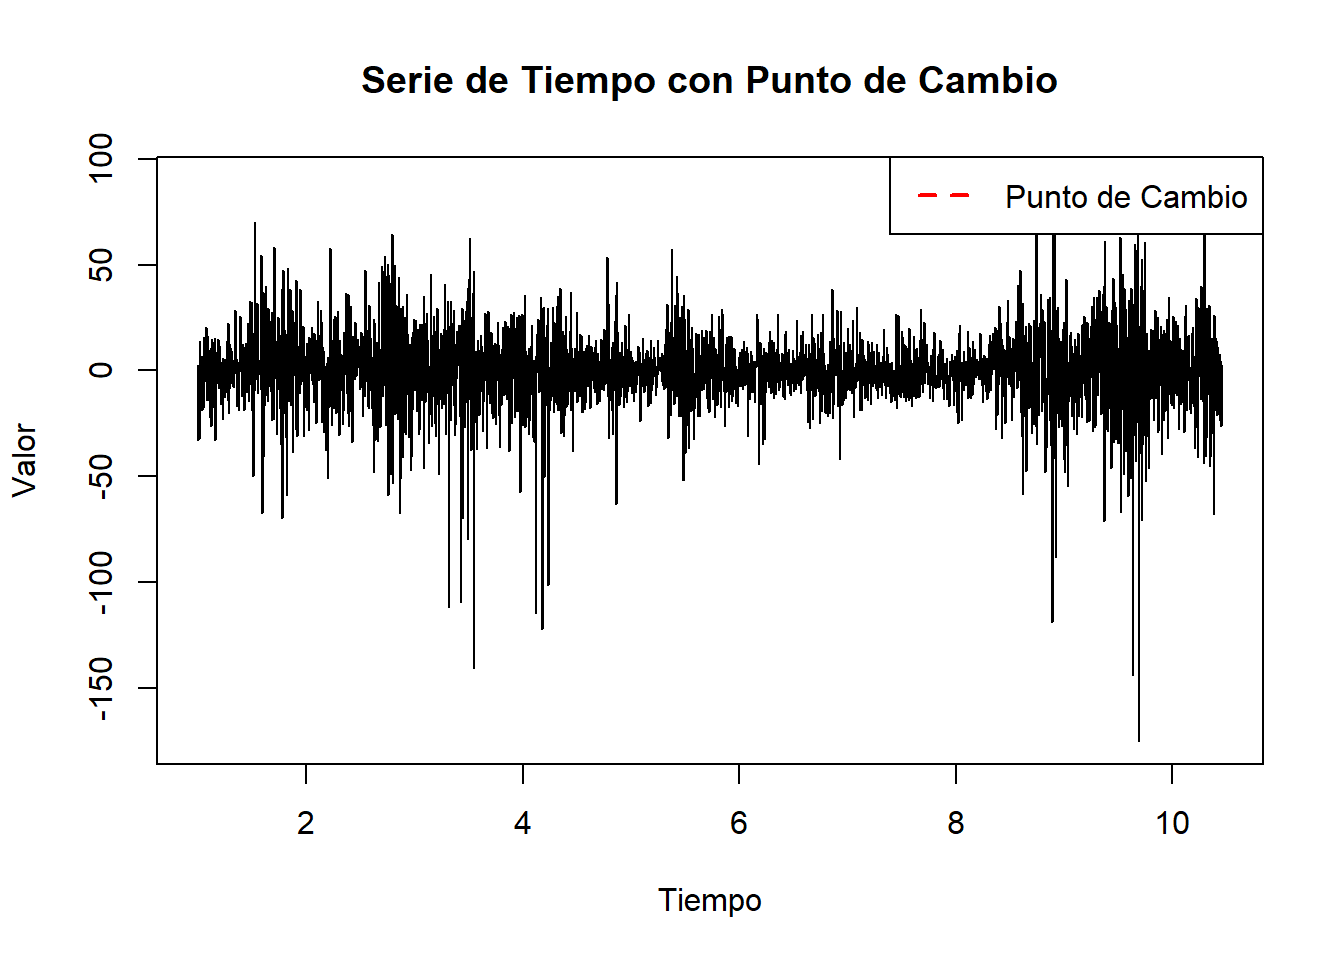
\includegraphics{bookdown-demo_files/figure-latex/unnamed-chunk-25-1.pdf}

\begin{Shaded}
\begin{Highlighting}[]
\NormalTok{pred}\OtherTok{\textless{}{-}}\FunctionTok{forecast}\NormalTok{(soybean\_ts,}\AttributeTok{h=}\DecValTok{12}\NormalTok{)}
\NormalTok{pred}
\end{Highlighting}
\end{Shaded}

\begin{verbatim}
##          Point Forecast     Lo 80    Hi 80     Lo 95    Hi 95
## 10.45753      -8.494463 -28.69910 11.71017 -39.39478 22.40586
## 10.46027       1.707605 -18.49703 21.91224 -29.19271 32.60792
## 10.46301      -1.862220 -22.06685 18.34241 -32.76254 29.03810
## 10.46575      -8.089611 -28.29424 12.11502 -38.98993 22.81071
## 10.46849       9.909409 -10.29522 30.11404 -20.99091 40.80973
## 10.47123       9.178946 -11.02569 29.38358 -21.72137 40.07927
## 10.47397       9.724160 -10.48047 29.92879 -21.17616 40.62448
## 10.47671       6.439264 -13.76537 26.64390 -24.46106 37.33958
## 10.47945      -7.246653 -27.45129 12.95798 -38.14697 23.65367
## 10.48219      -4.370599 -24.57523 15.83403 -35.27092 26.52972
## 10.48493       1.092988 -19.11165 21.29762 -29.80733 31.99331
## 10.48767      -6.704761 -26.90939 13.49987 -37.60508 24.19556
\end{verbatim}

\begin{Shaded}
\begin{Highlighting}[]
\FunctionTok{plot}\NormalTok{(pred, }\AttributeTok{main=}\StringTok{" "}\NormalTok{, }\AttributeTok{ylab=}\StringTok{"valor"}\NormalTok{, }\AttributeTok{col=}\StringTok{"deepskyblue"}\NormalTok{, }\AttributeTok{xlab=}\StringTok{"Tiempo"}\NormalTok{)}
\FunctionTok{title}\NormalTok{(}\AttributeTok{main=}\StringTok{"Predicción DIF Precios del aceite de soya"}\NormalTok{)}
\end{Highlighting}
\end{Shaded}

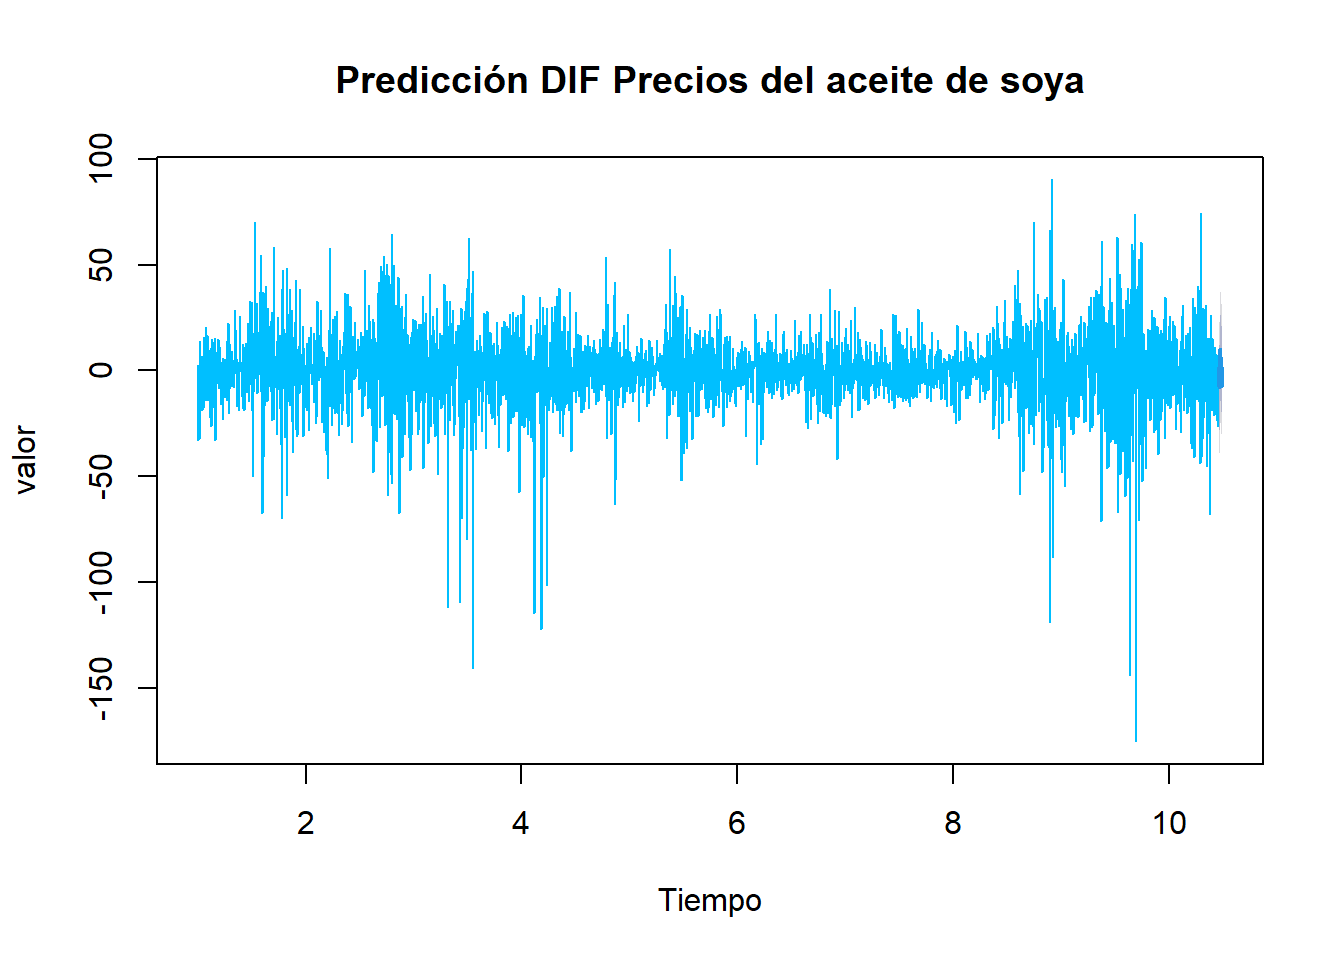
\includegraphics{bookdown-demo_files/figure-latex/unnamed-chunk-27-1.pdf}

\hypertarget{final-words}{%
\chapter{Final Words}\label{final-words}}

We have finished a nice book.

  \bibliography{book.bib,packages.bib}

\end{document}
